% Options for packages loaded elsewhere
\PassOptionsToPackage{unicode}{hyperref}
\PassOptionsToPackage{hyphens}{url}
%
\documentclass[
]{book}
\title{R Reference Manual}
\author{}
\date{\vspace{-2.5em}}

\usepackage{amsmath,amssymb}
\usepackage{lmodern}
\usepackage{iftex}
\ifPDFTeX
  \usepackage[T1]{fontenc}
  \usepackage[utf8]{inputenc}
  \usepackage{textcomp} % provide euro and other symbols
\else % if luatex or xetex
  \usepackage{unicode-math}
  \defaultfontfeatures{Scale=MatchLowercase}
  \defaultfontfeatures[\rmfamily]{Ligatures=TeX,Scale=1}
\fi
% Use upquote if available, for straight quotes in verbatim environments
\IfFileExists{upquote.sty}{\usepackage{upquote}}{}
\IfFileExists{microtype.sty}{% use microtype if available
  \usepackage[]{microtype}
  \UseMicrotypeSet[protrusion]{basicmath} % disable protrusion for tt fonts
}{}
\makeatletter
\@ifundefined{KOMAClassName}{% if non-KOMA class
  \IfFileExists{parskip.sty}{%
    \usepackage{parskip}
  }{% else
    \setlength{\parindent}{0pt}
    \setlength{\parskip}{6pt plus 2pt minus 1pt}}
}{% if KOMA class
  \KOMAoptions{parskip=half}}
\makeatother
\usepackage{xcolor}
\IfFileExists{xurl.sty}{\usepackage{xurl}}{} % add URL line breaks if available
\IfFileExists{bookmark.sty}{\usepackage{bookmark}}{\usepackage{hyperref}}
\hypersetup{
  pdftitle={R Reference Manual},
  hidelinks,
  pdfcreator={LaTeX via pandoc}}
\urlstyle{same} % disable monospaced font for URLs
\usepackage{color}
\usepackage{fancyvrb}
\newcommand{\VerbBar}{|}
\newcommand{\VERB}{\Verb[commandchars=\\\{\}]}
\DefineVerbatimEnvironment{Highlighting}{Verbatim}{commandchars=\\\{\}}
% Add ',fontsize=\small' for more characters per line
\usepackage{framed}
\definecolor{shadecolor}{RGB}{248,248,248}
\newenvironment{Shaded}{\begin{snugshade}}{\end{snugshade}}
\newcommand{\AlertTok}[1]{\textcolor[rgb]{0.94,0.16,0.16}{#1}}
\newcommand{\AnnotationTok}[1]{\textcolor[rgb]{0.56,0.35,0.01}{\textbf{\textit{#1}}}}
\newcommand{\AttributeTok}[1]{\textcolor[rgb]{0.77,0.63,0.00}{#1}}
\newcommand{\BaseNTok}[1]{\textcolor[rgb]{0.00,0.00,0.81}{#1}}
\newcommand{\BuiltInTok}[1]{#1}
\newcommand{\CharTok}[1]{\textcolor[rgb]{0.31,0.60,0.02}{#1}}
\newcommand{\CommentTok}[1]{\textcolor[rgb]{0.56,0.35,0.01}{\textit{#1}}}
\newcommand{\CommentVarTok}[1]{\textcolor[rgb]{0.56,0.35,0.01}{\textbf{\textit{#1}}}}
\newcommand{\ConstantTok}[1]{\textcolor[rgb]{0.00,0.00,0.00}{#1}}
\newcommand{\ControlFlowTok}[1]{\textcolor[rgb]{0.13,0.29,0.53}{\textbf{#1}}}
\newcommand{\DataTypeTok}[1]{\textcolor[rgb]{0.13,0.29,0.53}{#1}}
\newcommand{\DecValTok}[1]{\textcolor[rgb]{0.00,0.00,0.81}{#1}}
\newcommand{\DocumentationTok}[1]{\textcolor[rgb]{0.56,0.35,0.01}{\textbf{\textit{#1}}}}
\newcommand{\ErrorTok}[1]{\textcolor[rgb]{0.64,0.00,0.00}{\textbf{#1}}}
\newcommand{\ExtensionTok}[1]{#1}
\newcommand{\FloatTok}[1]{\textcolor[rgb]{0.00,0.00,0.81}{#1}}
\newcommand{\FunctionTok}[1]{\textcolor[rgb]{0.00,0.00,0.00}{#1}}
\newcommand{\ImportTok}[1]{#1}
\newcommand{\InformationTok}[1]{\textcolor[rgb]{0.56,0.35,0.01}{\textbf{\textit{#1}}}}
\newcommand{\KeywordTok}[1]{\textcolor[rgb]{0.13,0.29,0.53}{\textbf{#1}}}
\newcommand{\NormalTok}[1]{#1}
\newcommand{\OperatorTok}[1]{\textcolor[rgb]{0.81,0.36,0.00}{\textbf{#1}}}
\newcommand{\OtherTok}[1]{\textcolor[rgb]{0.56,0.35,0.01}{#1}}
\newcommand{\PreprocessorTok}[1]{\textcolor[rgb]{0.56,0.35,0.01}{\textit{#1}}}
\newcommand{\RegionMarkerTok}[1]{#1}
\newcommand{\SpecialCharTok}[1]{\textcolor[rgb]{0.00,0.00,0.00}{#1}}
\newcommand{\SpecialStringTok}[1]{\textcolor[rgb]{0.31,0.60,0.02}{#1}}
\newcommand{\StringTok}[1]{\textcolor[rgb]{0.31,0.60,0.02}{#1}}
\newcommand{\VariableTok}[1]{\textcolor[rgb]{0.00,0.00,0.00}{#1}}
\newcommand{\VerbatimStringTok}[1]{\textcolor[rgb]{0.31,0.60,0.02}{#1}}
\newcommand{\WarningTok}[1]{\textcolor[rgb]{0.56,0.35,0.01}{\textbf{\textit{#1}}}}
\usepackage{longtable,booktabs,array}
\usepackage{calc} % for calculating minipage widths
% Correct order of tables after \paragraph or \subparagraph
\usepackage{etoolbox}
\makeatletter
\patchcmd\longtable{\par}{\if@noskipsec\mbox{}\fi\par}{}{}
\makeatother
% Allow footnotes in longtable head/foot
\IfFileExists{footnotehyper.sty}{\usepackage{footnotehyper}}{\usepackage{footnote}}
\makesavenoteenv{longtable}
\usepackage{graphicx}
\makeatletter
\def\maxwidth{\ifdim\Gin@nat@width>\linewidth\linewidth\else\Gin@nat@width\fi}
\def\maxheight{\ifdim\Gin@nat@height>\textheight\textheight\else\Gin@nat@height\fi}
\makeatother
% Scale images if necessary, so that they will not overflow the page
% margins by default, and it is still possible to overwrite the defaults
% using explicit options in \includegraphics[width, height, ...]{}
\setkeys{Gin}{width=\maxwidth,height=\maxheight,keepaspectratio}
% Set default figure placement to htbp
\makeatletter
\def\fps@figure{htbp}
\makeatother
\setlength{\emergencystretch}{3em} % prevent overfull lines
\providecommand{\tightlist}{%
  \setlength{\itemsep}{0pt}\setlength{\parskip}{0pt}}
\setcounter{secnumdepth}{5}
\usepackage{booktabs}
\ifLuaTeX
  \usepackage{selnolig}  % disable illegal ligatures
\fi
\usepackage[]{natbib}
\bibliographystyle{apalike}

\begin{document}
\maketitle

{
\setcounter{tocdepth}{1}
\tableofcontents
}
\hypertarget{introduction}{%
\chapter{Introduction}\label{introduction}}

In \emph{R for Data Science}, Garrett Grolemund and Hadley Wickham outline the tools needed to tackle about 80\% of the tasks required in a typical data science project (``\href{https://r4ds.had.co.nz/introduction.html}{Introduction}''). Those tools, illustrated in the diagram below and the organizing template for this reference manual, are:

\begin{itemize}
\tightlist
\item
  Import
\item
  Tidy
\item
  Transform
\item
  Visualize
\item
  Model
\item
  Communicate
\item
  Program
\end{itemize}

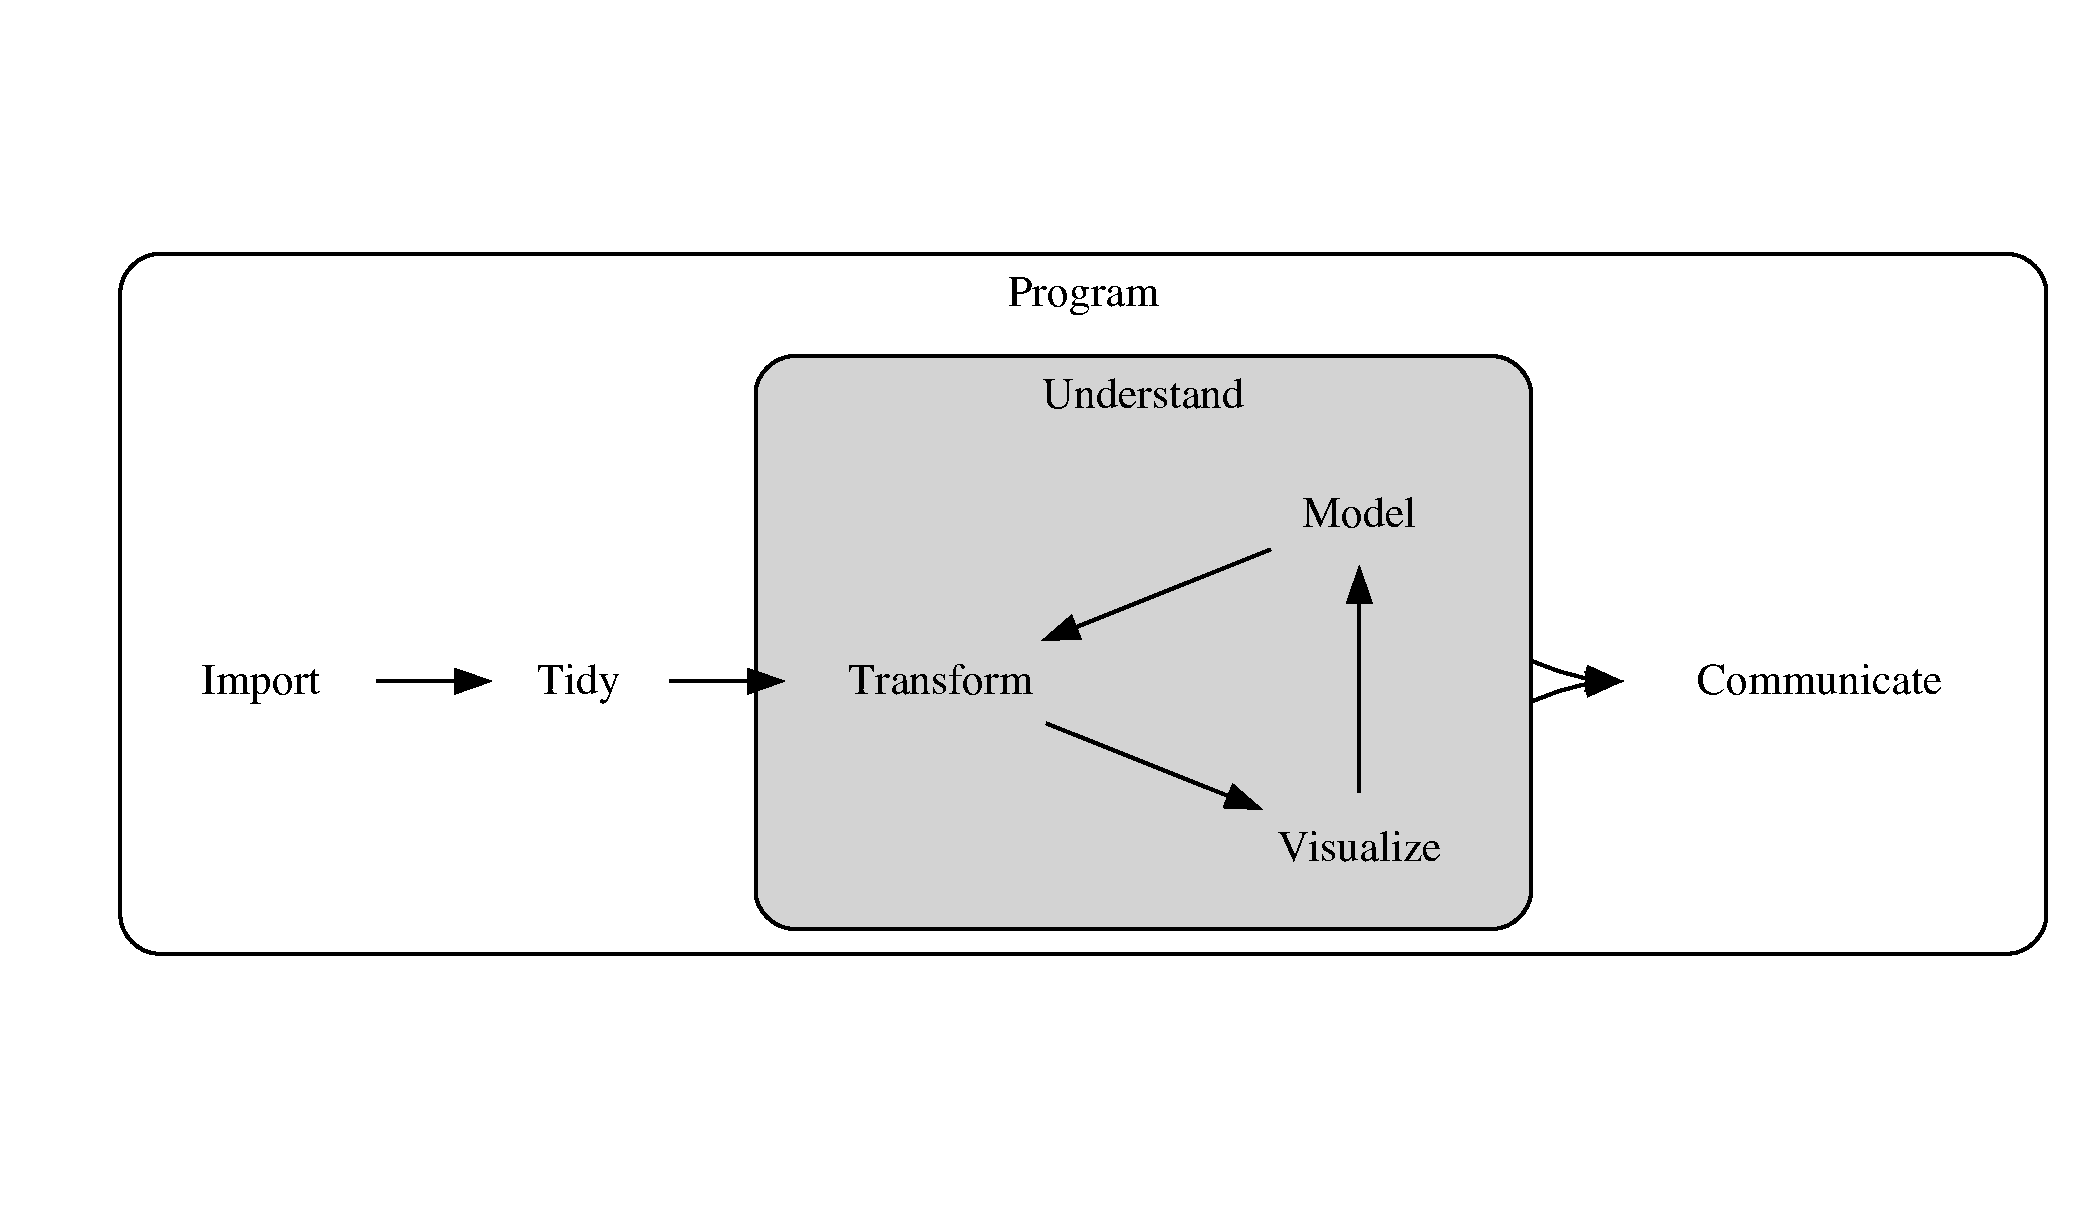
\includegraphics{R_Reference_Manual_files/figure-latex/unnamed-chunk-1-1.pdf}

\hypertarget{references-resources}{%
\section{References \& Resources}\label{references-resources}}

\begin{itemize}
\item
  For an introduction to the R programming language, see the R Project for Statistical Computing's \href{https://www.r-project.org/about.html}{``What is R?''} and Wikipedia's \href{https://en.wikipedia.org/wiki/R_(programming_language)}{``R (programming language).''}
\item
  To download R, go to \href{https://www.r-project.org/}{r-project.org} and choose the cloud CRAN Mirror option.
\item
  To program in the R language on a user-friendly platform, download the \href{https://www.rstudio.com/}{RStudio} IDE.
\item
  \href{https://www.r-project.org/}{The R Project for Statistical Computing}

  \begin{itemize}
  \tightlist
  \item
    \href{https://cran.r-project.org/web/packages/}{Library of R Packages}
  \item
    \href{https://www.r-project.org/help.html}{\emph{Getting Help with R}}
  \item
    \href{https://cran.r-project.org/manuals.html}{\emph{The R Manuals}}
  \item
    \href{https://cran.r-project.org/faqs.html}{\emph{Frequently Asked Questions}}
  \item
    \href{https://www.r-project.org/doc/bib/R-books.html}{\emph{Books Related to R}}
  \item
    \href{https://www.r-project.org/other-docs.html}{\emph{Documentation}}
  \end{itemize}
\item
  \href{https://www.rstudio.com/}{RStudio}

  \begin{itemize}
  \tightlist
  \item
    \href{https://www.rstudio.com/resources/cheatsheets/}{\emph{RStudio Cheat Sheets}}
  \item
    \href{https://www.rstudio.com/resources/webinars/}{\emph{Webinars and Videos On Demand}}
  \item
    \href{https://www.rstudio.com/online-learning/}{\emph{Online learning}}
  \item
    \href{https://blog.rstudio.com/}{\emph{RStudio Blog}}
  \end{itemize}
\item
  Online Manuals

  \begin{itemize}
  \tightlist
  \item
    \href{http://r4ds.had.co.nz/}{\emph{R for Data Science}}
  \item
    \href{http://adv-r.had.co.nz/}{\emph{Advanced R}} by Hadley Wickham
    + Hadley's second edition draft is available \href{https://adv-r.hadley.nz/}{here}.
  \item
    \href{http://r-pkgs.had.co.nz/}{\emph{R Packages}} by Hadley Wickham
  \item
    \href{http://www.burns-stat.com/pages/Tutor/R_inferno.pdf}{\emph{The R Inferno}} by Patrick Burns
  \item
    \href{http://style.tidyverse.org/}{\emph{The tidyverse style guide}}
  \item
    \href{https://bookdown.org/csgillespie/efficientR/}{\emph{Efficient R Programming}}
  \item
    \href{https://committedtotape.shinyapps.io/freeR/}{\emph{Free R Reading Material}}
  \item
    \href{https://rstats.wtf/}{\emph{What They Forgot to Teach You About R}} by Jenny Bryan and Jim Hester
  \end{itemize}
\item
  Other Online Resources

  \begin{itemize}
  \tightlist
  \item
    \href{https://www.datacamp.com/}{DataCamp}
  \item
    \href{https://www.rdocumentation.org/}{RDocumentation}
  \item
    \href{https://www.r-bloggers.com/how-to-learn-r-2/}{R Bloggers}

    \begin{itemize}
    \tightlist
    \item
      \href{https://www.r-bloggers.com/how-to-learn-r-2/}{``Tutorials for learning R''}
    \end{itemize}
  \item
    \href{https://regex101.com/}{Regular Expressions 101}
  \end{itemize}
\end{itemize}

\hypertarget{import-or-create-data}{%
\chapter{Import or Create Data}\label{import-or-create-data}}

\hypertarget{create-data}{%
\section{Create Data}\label{create-data}}

\texttt{\{base\}}

\begin{itemize}
\tightlist
\item
  \texttt{array()}
\item
  \texttt{c()}

  \begin{itemize}
  \tightlist
  \item
    See \texttt{base::vector()}.
  \end{itemize}
\item
  \texttt{data.frame()}
\item
  \texttt{dir.create()}
\item
  \texttt{factor()}
\item
  \texttt{list()}
\item
  \texttt{matrix()}
\item
  \texttt{seq()}
\item
  \texttt{vector()}

  \begin{itemize}
  \tightlist
  \item
    Preferable to \texttt{base::c()} when creating an empty vector (\href{https://www.datacamp.com/community/tutorials/five-tips-r-code-improve}{``Five Tips to Improve Your R Code''}).
  \end{itemize}
\end{itemize}

\texttt{\{stats\}}

\begin{itemize}
\tightlist
\item
  \texttt{dnorm()}
\item
  \texttt{pnorm()}
\item
  \texttt{qnorm()}
\item
  \texttt{rnorm()}
\end{itemize}

\texttt{\{tibble\}}

\begin{itemize}
\tightlist
\item
  \texttt{add\_row()}
\item
  \texttt{tibble()}
\item
  \texttt{tribble()}
\end{itemize}

\hypertarget{local-drive}{%
\section{Local Drive}\label{local-drive}}

\texttt{\{base\}}

\begin{itemize}
\tightlist
\item
  \texttt{attach()}

  \begin{itemize}
  \tightlist
  \item
    Allows objects in the database to be accessed by giving their names (e.g., \texttt{height} rather than \texttt{women\$height}).
  \end{itemize}
\item
  \texttt{file.choose()}
\item
  \texttt{file.size()}
\item
  \texttt{load()}

  \begin{itemize}
  \tightlist
  \item
    Reload datasets saved with \texttt{base::save()}.
  \end{itemize}
\item
  \texttt{readRDS()}

  \begin{itemize}
  \tightlist
  \item
    Restore an R object written with \texttt{base::saveRDS()}.
  \end{itemize}
\end{itemize}

\texttt{\{data.table\}}

\begin{itemize}
\tightlist
\item
  \texttt{fread()}

  \begin{itemize}
  \tightlist
  \item
    Similar to \texttt{utils::read.table()}, but faster and more convenient for large data sets.
  \end{itemize}
\end{itemize}

\texttt{\{foreign\}}

\begin{itemize}
\tightlist
\item
  \texttt{read.spss()}
\end{itemize}

\texttt{\{haven\}}

\begin{itemize}
\tightlist
\item
  \texttt{read\_sas()}
\end{itemize}

\texttt{\{readr\}}

\begin{itemize}
\tightlist
\item
  \texttt{read\_csv()}
\item
  \texttt{read\_csv2()}
\item
  \texttt{read\_delim()}

  \begin{itemize}
  \tightlist
  \item
    Remove imported attributes using \texttt{\%\textgreater{}\%\ .{[}{]}}, \texttt{attr(df,\ "spec")\ \textless{}-\ NULL}, or \texttt{\%\textgreater{}\%\ data.frame()}.
  \end{itemize}
\item
  \texttt{read\_tsv()}
\end{itemize}

\texttt{\{readxl\}}

\begin{itemize}
\tightlist
\item
  \texttt{excel\_sheets()}
\item
  \texttt{read\_excel()}
\item
  \texttt{read\_xls()}
\item
  \texttt{read\_xlsx()}
\end{itemize}

\texttt{\{utils\}}

\begin{itemize}
\tightlist
\item
  \texttt{data()}

  \begin{itemize}
  \tightlist
  \item
    Load specified data sets, or list the available data sets.
  \item
    Use this function to load the data sets that accompany R packages, such as \texttt{openintro::hsb2}, \texttt{openintro::email50},and \texttt{gapminder::gapminder}.
  \end{itemize}
\item
  \texttt{read.csv()}
\item
  \texttt{read.csv2()}
\item
  \texttt{read.delim()}
\item
  \texttt{read.delim2()}
\item
  \texttt{read.table()}
\end{itemize}

\texttt{\{XLConnect\}}

\begin{itemize}
\tightlist
\item
  \texttt{readWorksheetFromFile()}
\end{itemize}

\hypertarget{internet}{%
\section{Internet}\label{internet}}

\texttt{\{httr\}}

\begin{itemize}
\tightlist
\item
  \texttt{GET()}

  \begin{itemize}
  \tightlist
  \item
    Get a URL.
  \end{itemize}
\end{itemize}

\texttt{\{jsonlite\}}

\begin{itemize}
\tightlist
\item
  \texttt{read\_json()}
\end{itemize}

\texttt{\{readr\}}

\begin{itemize}
\tightlist
\item
  \texttt{read\_csv()}
\item
  \texttt{read\_csv2()}
\item
  \texttt{read\_delim()}
\item
  \texttt{read\_tsv()}
\end{itemize}

\texttt{\{rjson\}}

\begin{itemize}
\tightlist
\item
  \texttt{fromJSON()}

  \begin{itemize}
  \tightlist
  \item
    Convert JSON to R.
  \end{itemize}
\end{itemize}

\texttt{\{utils\}}

\begin{itemize}
\tightlist
\item
  \texttt{download.file()}

  \begin{itemize}
  \tightlist
  \item
    See example below.
  \end{itemize}
\item
  \texttt{unzip()}

  \begin{itemize}
  \tightlist
  \item
    See example below.
  \end{itemize}
\end{itemize}

\hypertarget{examples}{%
\subsection{Examples}\label{examples}}

\texttt{utils::download.file()}:

\begin{Shaded}
\begin{Highlighting}[]
\FunctionTok{download.file}\NormalTok{(}
  \StringTok{"https://assets.datacamp.com/production/repositories/5028/datasets/a55843f83746968c7f118d82ed727db9c71e891f/snake\_river\_visits.rds"}\NormalTok{,}
  \AttributeTok{destfile =} \FunctionTok{paste0}\NormalTok{(}\FunctionTok{getwd}\NormalTok{(), }\StringTok{"/Snake River Visits.rds"}\NormalTok{)}
\NormalTok{)}

\CommentTok{\# Option 1:}
\NormalTok{snake\_river\_visits }\OtherTok{\textless{}{-}} \FunctionTok{readRDS}\NormalTok{(}\FunctionTok{file.choose}\NormalTok{())}

\CommentTok{\# Option 2:}
\NormalTok{snake\_river\_path   }\OtherTok{\textless{}{-}} \FunctionTok{paste0}\NormalTok{(}\FunctionTok{getwd}\NormalTok{(), }\StringTok{"/Snake River Visits.rds"}\NormalTok{)}
\NormalTok{snake\_river\_visits }\OtherTok{\textless{}{-}} \FunctionTok{readRDS}\NormalTok{(snake\_river\_path)}
\end{Highlighting}
\end{Shaded}

\texttt{utils::download.file()} for .Rdata files:

\begin{Shaded}
\begin{Highlighting}[]
\CommentTok{\# Example 1:}
\FunctionTok{download.file}\NormalTok{(}
  \StringTok{"https://assets.datacamp.com/production/repositories/236/datasets/7f714f993f1ad4c3d26412ae1e537ce6355b1b54/iris.RData"}\NormalTok{, }
  \AttributeTok{destfile =} \StringTok{"datacamp\_iris\_dataset.Rdata"}
\NormalTok{)}

\FunctionTok{load}\NormalTok{(}\StringTok{"datacamp\_iris\_dataset.Rdata"}\NormalTok{)}

\CommentTok{\# Example 2:}
\FunctionTok{download.file}\NormalTok{(}
  \StringTok{"https://assets.datacamp.com/production/repositories/235/datasets/3b6fc2923b599058584b57d8c605c6bef454d273/CHIS2009\_reduced\_2.Rdata"}\NormalTok{,}
  \AttributeTok{destfile =} \StringTok{"chis\_2009.Rdata"}\NormalTok{,}
  \CommentTok{\# The documentation for \textasciigrave{}download.file\textasciigrave{} indicates that the function will}
  \CommentTok{\# automatically include \textasciigrave{}mode = "wb"\textasciigrave{} for .Rdata files. That may have happened}
  \CommentTok{\# in Example 1, but didn\textquotesingle{}t happen in Example 2, which is why I\textquotesingle{}ve included it.}
  \AttributeTok{mode =} \StringTok{"wb"}
\NormalTok{)}

\FunctionTok{load}\NormalTok{(}\StringTok{"chis\_2009.Rdata"}\NormalTok{)}
\end{Highlighting}
\end{Shaded}

\texttt{utils::unzip()}:

\begin{Shaded}
\begin{Highlighting}[]
\FunctionTok{download.file}\NormalTok{(}
  \StringTok{"https://assets.datacamp.com/production/repositories/1069/datasets/578834f5908e3b2fa575429a287586d1eaeb2e54/countries2.zip"}\NormalTok{,}
  \AttributeTok{destfile =} \StringTok{"Data Sets/Countries"}\NormalTok{,}
  \AttributeTok{mode =} \StringTok{"wb"}
\NormalTok{)}

\FunctionTok{unzip}\NormalTok{(}\StringTok{"Data Sets/Countries"}\NormalTok{, }\AttributeTok{exdir =} \StringTok{"Data Sets"}\NormalTok{)}
\end{Highlighting}
\end{Shaded}

\hypertarget{database}{%
\section{Database}\label{database}}

\texttt{\{DBI\}}

\begin{itemize}
\tightlist
\item
  \texttt{dbAppendTable()}
\item
  \texttt{dbBind()}
\item
  \texttt{dbClearResult()}
\item
  \texttt{dbConnect()}
\item
  \texttt{dbCreateTable()}
\item
  \texttt{dbDataType()}
\item
  \texttt{dbDisconnect()}
\item
  \texttt{dbExecute()}
\item
  \texttt{dbFetch()}
\item
  \texttt{dbGetQuery()}
\item
  \texttt{dbListTables()}

  \begin{itemize}
  \tightlist
  \item
    Specify schema with \texttt{dbListTables(conn,\ schema\ =\ "schema\_name")}.
  \end{itemize}
\item
  \texttt{dbReadTable()}
\item
  \texttt{dbRemoveTable()}
\item
  \texttt{dbSendQuery()}
\item
  \texttt{dbSendStatement()}
\item
  \texttt{Id()}

  \begin{itemize}
  \tightlist
  \item
    See example below.
  \end{itemize}
\item
  \texttt{SQL()}

  \begin{itemize}
  \tightlist
  \item
    See example below.
  \end{itemize}
\end{itemize}

\texttt{\{dbplyr\}}

\begin{itemize}
\tightlist
\item
  \texttt{in\_schema()}
\item
  \texttt{tbl()}
\end{itemize}

\texttt{\{odbc\}}

\begin{itemize}
\tightlist
\item
  \texttt{dbConnect()}

  \begin{itemize}
  \tightlist
  \item
    See example below for specifying a database.
  \item
    See example below for troubleshooting hang-ups.
  \end{itemize}
\end{itemize}

\hypertarget{examples-1}{%
\subsection{Examples}\label{examples-1}}

\texttt{DBI::Id()} vs \texttt{DBI::SQL()}:

The following are comparable methods of accessing \texttt{\textless{}database\textgreater{}.\textless{}schema\_name\textgreater{}.\textless{}table\_name\textgreater{}}:

\begin{Shaded}
\begin{Highlighting}[]
\FunctionTok{dbCreateTable}\NormalTok{(}
\NormalTok{  conn,}
  \AttributeTok{name =} 
    \FunctionTok{Id}\NormalTok{(}\AttributeTok{catalog =} \StringTok{"database\_name"}\NormalTok{, }\AttributeTok{schema =} \StringTok{"schema\_name"}\NormalTok{, }\AttributeTok{table =} \StringTok{"table\_name"}\NormalTok{),}
  \AttributeTok{fields =}\NormalTok{ sample\_data\_frame}
\NormalTok{)}

\FunctionTok{dbCreateTable}\NormalTok{(}
\NormalTok{  conn,}
  \AttributeTok{name =} \FunctionTok{SQL}\NormalTok{(}\StringTok{"database\_name.schema\_name.table\_name"}\NormalTok{),}
  \AttributeTok{fields =}\NormalTok{ sample\_data\_frame}
\NormalTok{)}
\end{Highlighting}
\end{Shaded}

\texttt{odbc::dbConnect()}:

\begin{Shaded}
\begin{Highlighting}[]
\CommentTok{\# Specify database:}
\NormalTok{conn\_1 }\OtherTok{\textless{}{-}} \FunctionTok{dbConnect}\NormalTok{(odbc}\SpecialCharTok{::}\FunctionTok{odbc}\NormalTok{(), }\AttributeTok{dsn =} \StringTok{"sql"}\NormalTok{) }\CommentTok{\# Default database: Actuary}

\NormalTok{conn\_2 }\OtherTok{\textless{}{-}} \FunctionTok{dbConnect}\NormalTok{(odbc}\SpecialCharTok{::}\FunctionTok{odbc}\NormalTok{(), }\AttributeTok{dsn =} \StringTok{"sql"}\NormalTok{, }\AttributeTok{Database =} \StringTok{"Staging"}\NormalTok{)}

\CommentTok{\# Troubleshoot hang{-}ups}
\CommentTok{\# It appears that RStudio\textquotesingle{}s attempt to load information into the Connection Pane,}
\CommentTok{\# via \textasciigrave{}odbc::dbConnect\textasciigrave{}, can sometimes cause the call to hang, indefinitely.}
\CommentTok{\# Use the following code to access the database in such a situation:}

\FunctionTok{options}\NormalTok{(}\AttributeTok{connectionObserver =} \ConstantTok{FALSE}\NormalTok{)}
\end{Highlighting}
\end{Shaded}

\hypertarget{references}{%
\subsection{References}\label{references}}

\begin{itemize}
\tightlist
\item
  \href{db.rstudio.com}{``Databases using R''}
\end{itemize}

\hypertarget{sql-and-r}{%
\subsection{SQL and R}\label{sql-and-r}}

\hypertarget{tips-and-troubleshooting-hints}{%
\subsubsection{Tips and Troubleshooting Hints}\label{tips-and-troubleshooting-hints}}

\begin{itemize}
\tightlist
\item
  Temp Tables

  \begin{itemize}
  \tightlist
  \item
    Use \texttt{SET\ NOCOUNT\ ON} in the SQL query to prevent R confusing the SQL rowcount return value with the temporary table.
  \end{itemize}
\item
  Try case-sensitive syntax (e.g., when querying a database other than the default).
\item
  Try selecting specific columns, rather than \texttt{SELECT\ *}, as SQL BLOB columns cause trouble.
\item
  Error Messages

  \begin{itemize}
  \tightlist
  \item
    \texttt{Error\ in\ env{[}{[}name{]}{]}\ \textless{}-\ x\ :\ attempt\ to\ use\ zero-length\ variable\ name}

    \begin{itemize}
    \tightlist
    \item
      Problem code: \texttt{select\ max(date)\ from\ table}
    \item
      Solution: \texttt{select\ max(date)\ as\ max\_date\ from\ table}
    \end{itemize}
  \item
    Error: ``Object does not exist or you do not have permission to create/delete it'' in combination with having db\_owner rights to the database.

    \begin{itemize}
    \tightlist
    \item
      Problem code: \texttt{CREATE\ OR\ ALTER\ PROCEDURE\ \textless{}non\_default\_schema\textgreater{}.\textless{}procedure\_name\textgreater{}}
    \item
      Solution: The default database in the ODBC is not set to the database you wish to modify. You can recreate the error in SSMS by using the same code (e.g.~set the database in the dropdown menu to master and run the script, which outputs the same error). Update the ODBC connection to specify the correct database.
    \end{itemize}
  \end{itemize}
\item
  Parameterized Queries

  \begin{itemize}
  \tightlist
  \item
    Reference: \href{https://db.rstudio.com/}{``Databases Using R''}
  \item
    See example below.
  \end{itemize}
\item
  Optimization:

  \begin{itemize}
  \tightlist
  \item
    \texttt{WHERE\ EXISTS} and \texttt{WHERE\ NOT\ EXISTS} are generally more efficient than \texttt{=} and \texttt{\textless{}\textgreater{}}.
  \item
    \texttt{=} is generally more efficient than \texttt{\textless{}\textgreater{}}.
  \end{itemize}
\end{itemize}

\hypertarget{examples-2}{%
\subsubsection{Examples}\label{examples-2}}

Parameterized query:

\begin{Shaded}
\begin{Highlighting}[]
\NormalTok{param\_query }\OtherTok{\textless{}{-}} \FunctionTok{dbSendQuery}\NormalTok{(con, }\StringTok{"select * from table where column = ?"}\NormalTok{)}

\FunctionTok{dbBind}\NormalTok{(param\_query, input)}
\FunctionTok{dbFetch}\NormalTok{(param\_query)}

\CommentTok{\# As a function:}
\NormalTok{query\_data }\OtherTok{\textless{}{-}} \ControlFlowTok{function}\NormalTok{(input) \{}
  
  \FunctionTok{dbBind}\NormalTok{(param\_query, input)}
  \FunctionTok{dbFetch}\NormalTok{(param\_query)}
\NormalTok{\}}

\FunctionTok{map}\NormalTok{(}\FunctionTok{as.list}\NormalTok{(df}\SpecialCharTok{$}\NormalTok{input\_column), query\_data) }\SpecialCharTok{\%\textgreater{}\%} \FunctionTok{bind\_rows}\NormalTok{()}
\end{Highlighting}
\end{Shaded}

\hypertarget{sql-references}{%
\subsubsection{SQL References}\label{sql-references}}

\begin{itemize}
\tightlist
\item
  \href{https://blog.jooq.org/2016/03/17/10-easy-steps-to-a-complete-understanding-of-sql/}{``10 Easy Steps to a Complete Understanding of SQL''}
\item
  \href{https://www.sqlite.org/queryplanner.html}{``Query Planning''}
\item
  \href{https://irene.rbind.io/post/using-sql-in-rstudio/}{``Using SQL in RStudio} by Irene Steves
\end{itemize}

\hypertarget{notes-references}{%
\section{Notes \& References}\label{notes-references}}

\begin{itemize}
\tightlist
\item
  \href{http://adv-r.had.co.nz/Data-structures.html}{``Data structures''} (Wickham, \href{http://adv-r.had.co.nz/}{\emph{Advanced R}})
\item
  \texttt{\{openintro\}} contains data sets useful for practicing and teaching.
\item
  \href{https://r4ds.had.co.nz/vectors.html}{``Vectors''} (Grolemund \& Wickham, \href{https://r4ds.had.co.nz/}{\emph{R for Data Science}})
\end{itemize}

\hypertarget{tidy}{%
\chapter{Tidy}\label{tidy}}

``Tidying your data means storing it in a consistent form that matches the semantics of the dataset with the way it is stored. In brief, when your data is tidy, each column is a variable and each row is an observation. Tidying data is important because the consistent structure lets you focus your struggle on questions about the data, not fighting to get the data into the right form for different functions.''\\
- Garrett Grolemund \& Hadley Wickham, \emph{R for Data Science}

\hypertarget{explore-raw-data}{%
\section{Explore Raw Data}\label{explore-raw-data}}

\texttt{\{base\}}

\begin{itemize}
\tightlist
\item
  \texttt{attr()}

  \begin{itemize}
  \tightlist
  \item
    \texttt{attr(x,\ "names")} is the same as \texttt{base::names(x)}.
  \item
    Use \texttt{attr(x,\ "names")\ \textless{}-\ value} to set attribute values.
  \end{itemize}
\item
  \texttt{attribute()}
\item
  \texttt{class()}
\item
  \texttt{colnames()}
\item
  \texttt{dim()}
\item
  \texttt{dimnames()}
\item
  \texttt{format()}
\item
  \texttt{length()}
\item
  \texttt{levels()}

  \begin{itemize}
  \tightlist
  \item
    Levels default to alphabetical order, so be careful when renaming them (i.e., don't accidentally set the ``F'' level equal to ``Male'' rather than ``Female'').
  \end{itemize}
\item
  \texttt{mode()}
\item
  \texttt{names()}
\item
  \texttt{nchar()}
\item
  \texttt{order()}
\item
  \texttt{rownames()}
\item
  \texttt{summary()}
\item
  \texttt{typeof()}
\end{itemize}

\texttt{\{graphics\}}

\begin{itemize}
\tightlist
\item
  \texttt{hist()}
\item
  \texttt{plot()}
\end{itemize}

\texttt{\{skimr\}}

\begin{itemize}
\tightlist
\item
  \texttt{skim()}

  \begin{itemize}
  \tightlist
  \item
    Similar to \texttt{tibble::glimpse()} and \texttt{utils::str()}.
  \end{itemize}
\end{itemize}

\texttt{\{tibble\}}

\begin{itemize}
\tightlist
\item
  \texttt{glimpse()}

  \begin{itemize}
  \tightlist
  \item
    Similar to \texttt{skimr::skim()} and \texttt{utils::str()}.
  \end{itemize}
\end{itemize}

\texttt{\{utils\}}

\begin{itemize}
\tightlist
\item
  \texttt{head()}
\item
  \texttt{str()}

  \begin{itemize}
  \tightlist
  \item
    Similar to \texttt{skimr::skim()} and \texttt{tibble::glimpse()}.
  \end{itemize}
\item
  \texttt{tail()}
\end{itemize}

\hypertarget{tidy-data}{%
\section{Tidy Data}\label{tidy-data}}

\texttt{\{base\}}

\begin{itemize}
\tightlist
\item
  \texttt{droplevels()}

  \begin{itemize}
  \tightlist
  \item
    Drop unused levels from factors.
  \item
    This function will keep levels that have even 1 or 2 counts. If you want to remove levels with low counts from a data set in order to simplify your analysis, first filter out those rows and then use \texttt{droplevels()}.
  \end{itemize}
\item
  \texttt{duplicated()}

  \begin{itemize}
  \tightlist
  \item
    See also \texttt{data.table::duplicated()}.
  \end{itemize}
\item
  \texttt{unique()}

  \begin{itemize}
  \tightlist
  \item
    See also \texttt{data.table::unique()}.
  \end{itemize}
\end{itemize}

\texttt{\{data.table\}}

\begin{itemize}
\tightlist
\item
  \texttt{anyDuplicated()}
\item
  \texttt{duplicated()}

  \begin{itemize}
  \tightlist
  \item
    See also \texttt{base::duplicated()}.
  \end{itemize}
\item
  \texttt{unique()}

  \begin{itemize}
  \tightlist
  \item
    See also \texttt{base::unique()}.
  \end{itemize}
\end{itemize}

\texttt{\{dplyr\}}

\begin{itemize}
\tightlist
\item
  \texttt{na\_if()}

  \begin{itemize}
  \tightlist
  \item
    See also \texttt{tidyr::replace\_na()}.
  \end{itemize}
\end{itemize}

\texttt{\{janitor\}}

\begin{itemize}
\tightlist
\item
  \texttt{clean\_names()}
\item
  \texttt{get\_dupes()}

  \begin{itemize}
  \tightlist
  \item
    Prefer over \texttt{base::duplicated()} and \texttt{data.table::duplicated()}.
  \end{itemize}
\item
  \texttt{remove\_empty()}
\end{itemize}

\texttt{\{naniar\}}

\begin{itemize}
\tightlist
\item
  \texttt{replace\_with\_na()}

  \begin{itemize}
  \tightlist
  \item
    Compliment to \texttt{tidyr::replace\_na()}; consider also \texttt{stringr::str\_replace(replacement\ =\ NA\_character\_)}.
  \end{itemize}
\end{itemize}

\texttt{\{purrr\}}

\begin{itemize}
\tightlist
\item
  \texttt{transpose()}

  \begin{itemize}
  \tightlist
  \item
    Turn a list-of-lists inside-out.
  \end{itemize}
\end{itemize}

\texttt{\{reshape2\}} (superseded by \texttt{\{tidyr\}})

\begin{itemize}
\tightlist
\item
  \texttt{cast()}

  \begin{itemize}
  \tightlist
  \item
    See \texttt{tidyr::pivot\_wider()}
  \end{itemize}
\item
  \texttt{melt()}

  \begin{itemize}
  \tightlist
  \item
    See \texttt{tidyr::pivot\_longer()}
  \end{itemize}
\end{itemize}

\texttt{\{splitstackshape\}}

\begin{itemize}
\tightlist
\item
  \texttt{cSplit()}

  \begin{itemize}
  \tightlist
  \item
    See also \texttt{tidyr::separate()}
  \end{itemize}
\end{itemize}

\texttt{\{tibble\}}

\begin{itemize}
\tightlist
\item
  \texttt{rowid\_to\_column()}

  \begin{itemize}
  \tightlist
  \item
    Add a column of sequential row IDs.
  \item
    Useful when a separate ID is required to manipulate rows or columns, such as when using \texttt{tidyr::pivot\_longe()r}
  \end{itemize}
\item
  \texttt{rownames\_to\_column()}
\end{itemize}

\texttt{\{tidyr\}}

\begin{itemize}
\tightlist
\item
  \texttt{fill()}

  \begin{itemize}
  \tightlist
  \item
    See \texttt{\{zoo\}}'s \texttt{na.fill()} and \texttt{na.locf()}.
  \end{itemize}
\item
  \texttt{nest()}

  \begin{itemize}
  \tightlist
  \item
    Nest repeated values in a list-variable.
  \item
    Helpful when separating a data frame in preparation to model the data for each grouping.
  \end{itemize}
\item
  \texttt{replace\_na()}

  \begin{itemize}
  \tightlist
  \item
    See \texttt{dplyr::na\_if()}.
  \end{itemize}
\item
  \texttt{separate()}
\item
  \texttt{pivot\_longer()}
\item
  \texttt{pivot\_wider()}
\item
  \texttt{unite()}
\item
  \texttt{unnest()}
\end{itemize}

\texttt{\{zoo\}}

\begin{itemize}
\tightlist
\item
  \texttt{na.fill()}
\item
  \texttt{na.locf()}

  \begin{itemize}
  \tightlist
  \item
    See \texttt{tidyr::fill()}.
  \end{itemize}
\end{itemize}

\hypertarget{prepare-data-for-analysis}{%
\section{Prepare Data for Analysis}\label{prepare-data-for-analysis}}

\hypertarget{coerce}{%
\subsection{Coerce}\label{coerce}}

\texttt{\{base\}}

\begin{itemize}
\tightlist
\item
  \texttt{as.array()}
\item
  \texttt{as.data.frame()}

  \begin{itemize}
  \tightlist
  \item
    See also\texttt{tibble::as\_tibble()}.
  \end{itemize}
\item
  \texttt{as.Date()}
\item
  \texttt{as.factor()}
\item
  \texttt{as.list()}
\item
  \texttt{as.matrix()}
\item
  \texttt{as.POSIX-()}
\item
  \texttt{factor()}

  \begin{itemize}
  \tightlist
  \item
    Rearrange the order of factors by using the \texttt{levels} argument. For example, rearrange the order of ``Bad,''Good,'' and ``Neutral'' using `levels = c(``Bad'', ``Neutral'', ``Good'').
  \end{itemize}
\item
  \texttt{is.na()}

  \begin{itemize}
  \tightlist
  \item
    Use \texttt{is.na\ \textless{}-} to set elements to \texttt{NA}.
  \end{itemize}
\item
  \texttt{unclass()}
\end{itemize}

\texttt{\{methods\}}

\begin{itemize}
\tightlist
\item
  \texttt{as()}
\end{itemize}

\texttt{\{tibble\}}

\begin{itemize}
\tightlist
\item
  \texttt{as\_tibble()}

  \begin{itemize}
  \tightlist
  \item
    Preferable to \texttt{base::as.data.frame()}.
  \end{itemize}
\item
  \texttt{enframe()}

  \begin{itemize}
  \tightlist
  \item
    Preferable to using \texttt{tibble::as\_tibble()} to coerce a vector to a data frame.
  \end{itemize}
\end{itemize}

\hypertarget{dates-and-datetimes}{%
\subsection{Dates and Datetimes}\label{dates-and-datetimes}}

\texttt{\{anytime\}}

\begin{itemize}
\tightlist
\item
  \texttt{anytime()}: Parse POSIXct or Date objects from input data.
\end{itemize}

\texttt{\{base\}}

\begin{itemize}
\tightlist
\item
  \texttt{as.Date()}
\item
  \texttt{OlsonNames()}

  \begin{itemize}
  \tightlist
  \item
    Displays available time zones.
  \end{itemize}
\item
  \texttt{as.POSIXct.*()}
\item
  \texttt{as.POSIXlt.*()}
\item
  \texttt{strptime()}

  \begin{itemize}
  \tightlist
  \item
    Date-time conversion to and from character.
  \end{itemize}
\item
  \texttt{Sys.timezone()}

  \begin{itemize}
  \tightlist
  \item
    See also \texttt{base::OlsonNames()}.
  \end{itemize}
\end{itemize}

\texttt{\{fasttime\}}

\begin{itemize}
\tightlist
\item
  \texttt{fastPOSIXct()}

  \begin{itemize}
  \tightlist
  \item
    Convert strings into \texttt{POSIXct} object (string must be in year, month, day, hour, minute, second format.)
  \end{itemize}
\end{itemize}

\texttt{\{hms\}}

\begin{itemize}
\tightlist
\item
  \texttt{as.hms()}
\item
  \texttt{hms()}

  \begin{itemize}
  \tightlist
  \item
    Store time-of-day values as \texttt{hms} class.
  \end{itemize}
\item
  \texttt{is.hms()}
\end{itemize}

\texttt{\{lubridate\}}

\begin{itemize}
\tightlist
\item
  \texttt{as\_date()}
\item
  \texttt{fast\_strptime()}

  \begin{itemize}
  \tightlist
  \item
    Fast C parser of numeric formats only that accepts explicit format arguments (just as \texttt{base::strptime()}).
  \item
    Note that the format argument must match the input exactly, including any non-white space characters (such as ``T'' and ``Z'').
  \end{itemize}
\item
  \texttt{make\_date()}

  \begin{itemize}
  \tightlist
  \item
    Create dates from numeric representations.
  \end{itemize}
\item
  \texttt{make\_datetime()}

  \begin{itemize}
  \tightlist
  \item
    Create date-times from numeric representations.
  \end{itemize}
\item
  \texttt{parse\_date\_time()}

  \begin{itemize}
  \tightlist
  \item
    This function can be slow, because it is designed to be forgiving and flexible. If the dates you are working with are in a consistent format (ideally ISO 8601), use one of the following: \texttt{fasttime::fastPOSIXct()} or \texttt{lubridate::parse\_date\_time2()}.
  \end{itemize}
\item
  \texttt{parse\_date\_time2()}

  \begin{itemize}
  \tightlist
  \item
    Fast C parser of numeric orders.
  \end{itemize}
\item
  \texttt{ymd()}: Parse dates with year, month, and day components.

  \begin{itemize}
  \tightlist
  \item
    Related formats: \texttt{ydm()}, \texttt{mdy()}, \texttt{myd()}, \texttt{dmy()}, \texttt{dym()}, \texttt{yq()}.
  \end{itemize}
\item
  \texttt{ymd\_hms()}: Parse date-times with year, month, day, hour, minute, and second components.

  \begin{itemize}
  \tightlist
  \item
    Related formats: \texttt{ymd\_hm()}, \texttt{ymd\_h()}, \texttt{dmy\_hms()}, \texttt{dmy\_hm()}, \texttt{dmy\_h()}, \texttt{mdy\_hms()}, \texttt{mdy\_hm()}, \texttt{mdy\_h()}, \texttt{ydm\_hms()}, \texttt{ydm\_hm()}, \texttt{ydm\_h()}.
  \end{itemize}
\end{itemize}

\hypertarget{filter}{%
\subsection{Filter}\label{filter}}

\texttt{\{dplyr\}}

\begin{itemize}
\tightlist
\item
  \texttt{filter()}
\end{itemize}

\texttt{\{purrr\}}

\begin{itemize}
\tightlist
\item
  \texttt{keep()}
\end{itemize}

\texttt{\{stats\}}

\begin{itemize}
\tightlist
\item
  \texttt{na.omit()}
\end{itemize}

\hypertarget{strings}{%
\subsection{Strings}\label{strings}}

\texttt{\{base\}}

\begin{itemize}
\tightlist
\item
  \texttt{agrep()}
\item
  \texttt{cat()}

  \begin{itemize}
  \tightlist
  \item
    Concatenate and print.
  \end{itemize}
\item
  \texttt{chartr()}

  \begin{itemize}
  \tightlist
  \item
    Change certain characters.
  \end{itemize}
\item
  \texttt{gregexpr()}
\item
  \texttt{grep()}
\item
  \texttt{grepl()}
\item
  \texttt{gsub()}
\item
  \texttt{regexec()}
\item
  \texttt{regexpr()}
\item
  \texttt{sub()}
\item
  \texttt{tolower()}

  \begin{itemize}
  \tightlist
  \item
    See also \texttt{stringr::str\_to\_lower()}.
  \end{itemize}
\item
  \texttt{toupper()}: Convert to uppercase.

  \begin{itemize}
  \tightlist
  \item
    See also \texttt{stringr::str\_to\_upper()}.
  \end{itemize}
\end{itemize}

\texttt{\{fuzzyjoin\}}

\begin{itemize}
\tightlist
\item
  \texttt{stringdist\_join()}
\item
  \texttt{stringdist\_anti\_join()}
\item
  \texttt{stringdist\_full\_join()}
\item
  \texttt{stringdist\_inner\_join()}
\item
  \texttt{stringdist\_left\_join()}
\item
  \texttt{stringdist\_right\_join()}
\item
  \texttt{stringdist\_semi\_join()}
\end{itemize}

\texttt{\{fuzzywuzzyR\}}

\begin{itemize}
\tightlist
\item
  \texttt{FuzzMatcher()}
\end{itemize}

\texttt{\{qdap\}}

\begin{itemize}
\tightlist
\item
  \texttt{check\_spelling()}
\end{itemize}

\texttt{\{qdapDictionaries\}}

\begin{itemize}
\tightlist
\item
  \texttt{DICTIONARY()}

  \begin{itemize}
  \tightlist
  \item
    Nettalk Corpus syllable data set.
  \end{itemize}
\item
  \texttt{GradyAugmented()}

  \begin{itemize}
  \tightlist
  \item
    Augmented list of Grady Ward's \emph{English Words} and Mark Kantrowitz's \emph{Names} List.
  \item
    Mark Kantrowitz's \emph{Names} list is available in full \href{http://www.cs.cmu.edu/afs/cs/project/ai-repository/ai/areas/nlp/corpora/names/}{here}.
  \end{itemize}
\end{itemize}

\texttt{\{stringr\}}

\begin{itemize}
\tightlist
\item
  \texttt{str\_detect}

  \begin{itemize}
  \tightlist
  \item
    Control the \texttt{pattern} argument options with \texttt{regex()} (e.g., \texttt{str\_detect(x,\ regex(pattern,\ ignore\_case\ =\ TRUE))}.
  \end{itemize}
\item
  \texttt{str\_remove()}
\item
  \texttt{str\_to\_lower()}
\item
  \texttt{str\_to\_title()}
\item
  \texttt{str\_trim()}
\item
  \texttt{str\_to\_upper()}
\end{itemize}

\hypertarget{test}{%
\subsection{Test}\label{test}}

\texttt{\{base\}}

\begin{itemize}
\tightlist
\item
  \texttt{all()}
\item
  \texttt{any()}

  \begin{itemize}
  \tightlist
  \item
    Use \texttt{any(is.na(data.frame))} to determine if there are any \texttt{NA} values in a data frame.
  \end{itemize}
\item
  \texttt{anyNA()}

  \begin{itemize}
  \tightlist
  \item
    Possibly faster implementation of \texttt{base::any(is.na(x))}.
  \end{itemize}
\item
  \texttt{exists()}
\item
  \texttt{is.array()}
\item
  \texttt{is.data.frame()}
\item
  \texttt{is.matrix()}
\item
  \texttt{is.vector()}
\item
  \texttt{setequal()}

  \begin{itemize}
  \tightlist
  \item
    Check two vectors for equality.
  \end{itemize}
\item
  \texttt{sum()}

  \begin{itemize}
  \tightlist
  \item
    Test whether all elements of a vector do or do not meet a certain condition, use as follows: \texttt{sum(email\$num\_char\ \textless{}\ 0)}.
  \end{itemize}
\end{itemize}

\texttt{\{purrr\}}

\begin{itemize}
\tightlist
\item
  \texttt{every()}
\end{itemize}

\texttt{\{stats\}}

\begin{itemize}
\tightlist
\item
  \texttt{complete.cases()}

  \begin{itemize}
  \tightlist
  \item
    Find complete cases (i.e., rows without \texttt{NA} values).
  \end{itemize}
\end{itemize}

\texttt{\{tibble\}}

\begin{itemize}
\tightlist
\item
  \texttt{is\_tibble()}
\end{itemize}

\hypertarget{transform}{%
\chapter{Transform}\label{transform}}

``Transformation includes narrowing in on observations of interest (like all people in one city, or all data from the last year), creating new variables that are functions of existing variables (like computing velocity from speed and time), and calculating a set of summary statistics (like counts or means).''\\
- Garrett Grolemund \& Hadley Wickham, \emph{R for Data Science}

\hypertarget{arithmetic-summary-statistics}{%
\section{Arithmetic \& Summary Statistics}\label{arithmetic-summary-statistics}}

\texttt{\{assertive\}}

\begin{itemize}
\tightlist
\item
  \texttt{is\_divisible\_by()}
\end{itemize}

\texttt{\{base\}}

\begin{itemize}
\tightlist
\item
  \texttt{abs()}
\item
  \texttt{colMeans()}
\item
  \texttt{colSums()}
\item
  \texttt{diff()}
\item
  \texttt{IQR()}
\item
  \texttt{max()}
\item
  \texttt{mean()}

  \begin{itemize}
  \tightlist
  \item
    Use \texttt{base::mean(variable\ ==\ value)} to calculate percentage match (accuracy); see example below.
  \end{itemize}
\item
  \texttt{median()}
\item
  \texttt{min()}
\item
  Mode: Use \texttt{table} to view the mode of a data set.
\item
  Operators:

  \begin{itemize}
  \tightlist
  \item
    Arithmetic Operators: \texttt{+}, \texttt{-}, \texttt{*}, \texttt{/}, \texttt{\%\%}
  \item
    Comparison Operators: \texttt{\textless{}}, \texttt{\textgreater{}}, \texttt{\textless{}=}, \texttt{\textgreater{}=}, \texttt{==}, \texttt{!=}.

    \begin{itemize}
    \tightlist
    \item
      Use \texttt{identical()} and \texttt{(all.equal))} rather than \texttt{==} and \texttt{!=} in tests where a single \texttt{TRUE} or \texttt{FALSE} is required (such as \texttt{if} expressions).
    \end{itemize}
  \end{itemize}
\item
  \texttt{range()}

  \begin{itemize}
  \tightlist
  \item
    Use \texttt{diff(range())} to get the range as a measure of variability.
  \end{itemize}
\item
  \texttt{round()}
\item
  \texttt{rowMeans()}
\item
  \texttt{rowSums()}
\item
  \texttt{scale()}
\item
  \texttt{sd()}
\item
  \texttt{signif()}

  \begin{itemize}
  \tightlist
  \item
    Round values to a specified number of significant digits.
  \end{itemize}
\item
  \texttt{sqrt()}
\item
  \texttt{sum()}
\item
  \texttt{summary()}
\item
  \texttt{var()}
\end{itemize}

\texttt{\{dplyr\}}

\begin{itemize}
\tightlist
\item
  \texttt{count()}
\item
  \texttt{group\_by()}
\item
  \texttt{n()}

  \begin{itemize}
  \tightlist
  \item
    Must be used within \texttt{summarize()}, \texttt{mutate()}, or \texttt{filter()}.
  \end{itemize}
\item
  \texttt{n\_distinct()}
\item
  \texttt{near()}

  \begin{itemize}
  \tightlist
  \item
    Compare two numeric vectors (safer than using \texttt{==}).
  \end{itemize}
\item
  \texttt{summarize()}

  \begin{itemize}
  \tightlist
  \item
    See \texttt{dplyr::n\_distinct()}.
  \end{itemize}
\item
  \texttt{tally()}
\item
  \texttt{top\_n()}
\end{itemize}

\texttt{\{dummies\}}

\begin{itemize}
\tightlist
\item
  \texttt{dummy.data.frame()}

  \begin{itemize}
  \tightlist
  \item
    Dummify a data frame (useful when needing to calculate the Jaccard index for categorical data)
  \end{itemize}
\end{itemize}

\texttt{\{magrittr\}}

\begin{itemize}
\tightlist
\item
  \texttt{extract()}

  \begin{itemize}
  \tightlist
  \item
    \texttt{x\ \%\textgreater{}\%\ extract(y)} is equivalent to \texttt{x{[}y{]}}.
  \end{itemize}
\item
  \texttt{extract2()}
\item
  \texttt{multiply\_by()}

  \begin{itemize}
  \tightlist
  \item
    \texttt{x\ \%\textgreater{}\%\ multiply\_by(y)} is equivalent to \texttt{x\ *\ y}.
  \end{itemize}
\item
  \texttt{raise\_to\_power()}

  \begin{itemize}
  \tightlist
  \item
    \texttt{x\ \%\textgreater{}\%\ raise\_to\_power(y)} is equivalent to \texttt{x\^{}y}.
  \end{itemize}
\end{itemize}

\texttt{\{stats\}}

\begin{itemize}
\tightlist
\item
  \texttt{aggregate()}

  \begin{itemize}
  \tightlist
  \item
    Compute summary statistics of data subsets.
  \end{itemize}
\item
  \texttt{cor()}
\item
  \texttt{cov()}
\item
  \texttt{cutree()}

  \begin{itemize}
  \tightlist
  \item
    Pair with \texttt{stats::hclust()}.
  \end{itemize}
\item
  \texttt{dist()}
\item
  \texttt{hclust()}
\item
  \texttt{lag()}
\item
  \texttt{rnorm()}
\item
  \texttt{var()}
\end{itemize}

\hypertarget{examples-3}{%
\subsection{Examples}\label{examples-3}}

\texttt{base::mean()}

\begin{Shaded}
\begin{Highlighting}[]
\NormalTok{by\_country }\OtherTok{\textless{}{-}} 
\NormalTok{  votes }\SpecialCharTok{\%\textgreater{}\%} 
  \FunctionTok{group\_by}\NormalTok{(country) }\SpecialCharTok{\%\textgreater{}\%} 
  \FunctionTok{summarize}\NormalTok{(}
    \AttributeTok{total =} \FunctionTok{n}\NormalTok{(),}
    \AttributeTok{percent\_yes =} \FunctionTok{mean}\NormalTok{(vote }\SpecialCharTok{==} \DecValTok{1}\NormalTok{))}

\CommentTok{\# Classification Trees: Compute the accuracy on the test dataset:}
\FunctionTok{mean}\NormalTok{(loans\_test}\SpecialCharTok{$}\NormalTok{outcome }\SpecialCharTok{==}\NormalTok{ loans\_test}\SpecialCharTok{$}\NormalTok{prediction)}
\end{Highlighting}
\end{Shaded}

\hypertarget{create-new-variables-or-modify-existing-ones}{%
\section{Create New Variables or Modify Existing Ones}\label{create-new-variables-or-modify-existing-ones}}

\texttt{countrycode}

\begin{itemize}
\tightlist
\item
  \texttt{countrycode()}: Convert country codes into country names.
\end{itemize}

\texttt{dplyr}

\begin{itemize}
\tightlist
\item
  \texttt{mutate()}: Add new variables.

  \begin{itemize}
  \tightlist
  \item
    \texttt{mutate()} can also be used to modify existing variables. To change the case of a character variable, for example, do something like:
  \item
    Child function: \texttt{transmute()} (drops existing variables).
  \end{itemize}
\item
  \texttt{recode()}: Recode values (the numeric alternative to using \texttt{if\_else} or \texttt{case\_when()}).
\end{itemize}

\textbf{Example:} \texttt{dplyr::mutate}

\begin{Shaded}
\begin{Highlighting}[]
\NormalTok{df }\OtherTok{\textless{}{-}}
\NormalTok{  df }\SpecialCharTok{\%\textgreater{}\%}
  \FunctionTok{mutate}\NormalTok{(}\AttributeTok{var\_name =} \FunctionTok{str\_to\_lower}\NormalTok{(var\_name))}

\CommentTok{\# Add a T/F vector, which can then be referenced to highlight certain }
\CommentTok{\# information in a plot:}

\NormalTok{df }\OtherTok{\textless{}{-}} 
\NormalTok{  df }\SpecialCharTok{\%\textgreater{}\%} 
  \FunctionTok{mutate}\NormalTok{(}\AttributeTok{hilight =} \AttributeTok{attributed\_provider\_id =} \DecValTok{95597}\NormalTok{)}
\end{Highlighting}
\end{Shaded}

\hypertarget{dates-and-datetimes-1}{%
\section{Dates and Datetimes}\label{dates-and-datetimes-1}}

\begin{itemize}
\tightlist
\item
  \texttt{base::date}

  \begin{itemize}
  \tightlist
  \item
    Get the current system date and time.
  \end{itemize}
\item
  \texttt{base::difftime}

  \begin{itemize}
  \tightlist
  \item
    Time intervals and differences.
  \item
    \texttt{base::difftime} is the function behind the \texttt{-} operator when used with dates and datetimes (e.g., \texttt{time\_1\ -\ time\_2} is equivalent to \texttt{difftime(time\_1,\ time\_2)}). The advantage of using \texttt{difftime} over \texttt{-}, however, is the \texttt{units} argument because it allows you to specify the unit of time in which the difference is calculated.
  \end{itemize}
\item
  \texttt{base::months}

  \begin{itemize}
  \tightlist
  \item
    Extract the month names.
  \end{itemize}
\item
  \texttt{base::quarters}

  \begin{itemize}
  \tightlist
  \item
    Extract the calendar quarters.
  \end{itemize}
\item
  \texttt{base::seq.Date}
\item
  \texttt{base::Sys.Date}

  \begin{itemize}
  \tightlist
  \item
    Get the current date in the current time zone.
  \end{itemize}
\item
  \texttt{base::Sys.time}

  \begin{itemize}
  \tightlist
  \item
    Get the absolute date-time value (which can be converted to various time zones and may return different days).
  \end{itemize}
\item
  \texttt{base::weekdays}

  \begin{itemize}
  \tightlist
  \item
    Extract weekday names.
  \end{itemize}
\item
  \texttt{lubridate::ceiling\_date}
\item
  \texttt{lubridate::date}

  \begin{itemize}
  \tightlist
  \item
    Get or set the date component of a date-time.
  \end{itemize}
\item
  \texttt{lubridate::day}

  \begin{itemize}
  \tightlist
  \item
    Get or set the day component of a datetime.
  \end{itemize}
\item
  \texttt{lubridate::floor\_date}
\item
  \texttt{lubridate::month}

  \begin{itemize}
  \tightlist
  \item
    Get or set the month component of a datetime.
  \end{itemize}
\item
  \texttt{lubridate::now}

  \begin{itemize}
  \tightlist
  \item
    The current time (as a POSIXct object).
  \end{itemize}
\item
  \texttt{lubridate::quarter}

  \begin{itemize}
  \tightlist
  \item
    Get or set the fiscal quarter or semester component of a datetime.
  \end{itemize}
\item
  \texttt{lubridate::round\_date}
\item
  Time spans: Duration

  \begin{itemize}
  \tightlist
  \item
    Use when you are interested in seconds elapsed.
  \item
    \texttt{lubridate::ddays}
  \item
    \texttt{lubridate::dhours}
  \item
    \texttt{lubridate::dminutes}
  \item
    \texttt{lubridate::dseconds}
  \item
    \texttt{lubridate::dweeks}
  \item
    \texttt{lubridate::dyears}
  \end{itemize}
\item
  Time spans: Interval

  \begin{itemize}
  \tightlist
  \item
    Use when you have a start and end.
  \item
    \texttt{\%-\/-\%}
  \item
    \texttt{int\_aligns}
  \item
    \texttt{int\_diff}
  \item
    \texttt{int\_end}
  \item
    \texttt{int\_flip}
  \item
    \texttt{int\_length}
  \item
    \texttt{int\_overlaps}
  \item
    \texttt{int\_shift}
  \item
    \texttt{int\_standardize}
  \item
    \texttt{int\_start}
  \item
    \texttt{interval}
  \item
    \texttt{is.interval}
  \end{itemize}
\item
  Time spans: Period

  \begin{itemize}
  \tightlist
  \item
    Use when you are interested in human units.
  \item
    \texttt{lubridate::day}
  \item
    \texttt{lubridate::hour}
  \item
    \texttt{lubridate::minute}
  \item
    \texttt{lubridate::month}
  \item
    \texttt{lubridate::second}
  \item
    \texttt{lubridate::week}
  \item
    \texttt{lubridate::year}
  \end{itemize}
\item
  Time zones:

  \begin{itemize}
  \tightlist
  \item
    \texttt{lubridate::force\_tz}

    \begin{itemize}
    \tightlist
    \item
      Change the time zone without changing the clock time.
    \end{itemize}
  \item
    \texttt{lubridate::tz}

    \begin{itemize}
    \tightlist
    \item
      Extract the time zone from a datetime.
    \end{itemize}
  \item
    \texttt{lubridate::with\_tz}

    \begin{itemize}
    \tightlist
    \item
      View the same instant in a different time zone.
    \end{itemize}
  \end{itemize}
\item
  \texttt{lubridate::today}
\item
  \texttt{lubridate::\%m+\%} \& \texttt{\%m-\%}

  \begin{itemize}
  \tightlist
  \item
    Add and subtract months to a date without exceeding the last day of the new month.
  \end{itemize}
\item
  \texttt{lubridate::\%within\%}

  \begin{itemize}
  \tightlist
  \item
    Test whether a date or interval falls within an interval.
  \end{itemize}
\item
  \texttt{lubridate::year}

  \begin{itemize}
  \tightlist
  \item
    Get or set the year component of a datetime.
  \end{itemize}
\end{itemize}

\hypertarget{factors}{%
\section{Factors}\label{factors}}

\texttt{forcats}

\begin{itemize}
\tightlist
\item
  \texttt{fct\_drop()}: Drop levels.
\item
  \texttt{fct\_reorder()}: Reorder levels, based on the value of another variable.
\item
  \texttt{fct\_rev()}: Reverse levels.
\end{itemize}

\texttt{stats}

\begin{itemize}
\tightlist
\item
  \texttt{reorder()}: Reorder levels of a factor.

  \begin{itemize}
  \tightlist
  \item
    Useful within the \texttt{aes()} argument in a \texttt{ggplot()} call.
  \end{itemize}
\end{itemize}

\hypertarget{merge-or-append-data}{%
\section{Merge or Append Data}\label{merge-or-append-data}}

\texttt{base}

\begin{itemize}
\tightlist
\item
  \texttt{append()}: Add elements to a vector.
\item
  \texttt{cbind()}: Combine objects by column.
\item
  \texttt{intersect()}: Combine data shared in common between two datasets.

  \begin{itemize}
  \tightlist
  \item
    Similar to \texttt{dplyr::semi\_join()}.
  \end{itemize}
\item
  \texttt{merge()}: Merge two data frames.

  \begin{itemize}
  \tightlist
  \item
    \texttt{dplyr::join} functions are an alternative to \texttt{merge()}.
  \end{itemize}
\item
  \texttt{rbind()}: Combine objects by row.
\item
  \texttt{setdiff()}: Find the difference between two vectors.

  \begin{itemize}
  \tightlist
  \item
    Similar to \texttt{dplyr::anti\_join()}.
  \end{itemize}
\item
  \texttt{union()}: Combine two datasets without duplicating values.
\end{itemize}

\texttt{dplyr}

\begin{itemize}
\tightlist
\item
  \texttt{bind()}: Bind multiple data frames by row and column.

  \begin{itemize}
  \tightlist
  \item
    Child functions: bind\_rows(), bind\_cols(), combine().
  \end{itemize}
\item
  Join Functions: Join two tables.

  \begin{itemize}
  \tightlist
  \item
    Filtering Joins:

    \begin{itemize}
    \tightlist
    \item
      anti\_join(): Return all rows from \texttt{x} where there are not matching values in \texttt{y}, keeping just columns from \texttt{x}.
    \item
      semi\_join(): Return all rows from \texttt{x} where there are matching values in \texttt{y}, keeping just columns from \texttt{x}. A semi join differs from an inner join because an inner join will return one row of \texttt{x} for each matching row of \texttt{y}, where a semi join will never duplicate rows of \texttt{x}.
    \item
      Mutating Joins:

      \begin{itemize}
      \tightlist
      \item
        full\_join(): Return all rows and all columns from both \texttt{x} and \texttt{y}. Where there are not matching values, returns \texttt{NA} for the one missing.
      \item
        inner\_join(): Return all rows from \texttt{x} where there are matching values in \texttt{y}, and all columns from \texttt{x} and \texttt{y}. If there are multiple matches between \texttt{x} and \texttt{y}, all combination of the matches are returned.
      \item
        left\_join(): Return all rows from \texttt{x}, and all columns from \texttt{x} and \texttt{y}. Rows in \texttt{x} with no match in \texttt{y} will have \texttt{NA} values in the new columns. If there are multiple matches between \texttt{x} and \texttt{y}, all combinations of the matches are returned.
      \item
        right\_join(): Return all rows from \texttt{y}, and all columns from \texttt{x} and \texttt{y}. Rows in \texttt{x} with no match in \texttt{y} will have \texttt{NA} values in the new columns. If there are multiple matches between \texttt{y} and \texttt{x}, all combinations of the matches are returned.
      \end{itemize}
    \end{itemize}
  \end{itemize}
\end{itemize}

\texttt{tibble}

\begin{itemize}
\tightlist
\item
  \texttt{add\_column()}: Add columns to a data frame.
\item
  \texttt{add\_row()}: Add rows to a data frame.
\end{itemize}

\hypertarget{narrow-in-on-observations-of-interest}{%
\section{Narrow in on Observations of Interest}\label{narrow-in-on-observations-of-interest}}

\texttt{\{base\}}

\begin{itemize}
\tightlist
\item
  \texttt{order()}

  \begin{itemize}
  \tightlist
  \item
    See also: \texttt{dplyr::arrange()}.
  \end{itemize}
\item
  \texttt{prop.table()}

  \begin{itemize}
  \tightlist
  \item
    Express table entries as proportions of the marginal table (thus, as the values are proportions of the whole, \texttt{sum(prop.table(table\_name))} = 1.)
  \item
    The input is a table produced by \texttt{base::table()}.
  \item
    Specify conditional proportions on rows or columns by using the \texttt{margin} argument.
  \end{itemize}
\item
  \texttt{table()}: Build a table of the counts at each combination of factor levels.

  \begin{itemize}
  \tightlist
  \item
    Use \texttt{base::prop.table()} to see the table entries expressed as proportions.
  \end{itemize}
\end{itemize}

\texttt{\{dplyr\}}

\begin{itemize}
\tightlist
\item
  \texttt{arrange()}
\item
  \texttt{distinct()}
\item
  \texttt{filter()}

  \begin{itemize}
  \tightlist
  \item
    When using multiple \texttt{\textbar{}} conditions, use \texttt{\%in\%} to save space; see example below.
  \end{itemize}
\item
  \texttt{rename()}
\item
  \texttt{sample\_n()}
\item
  \texttt{select()}

  \begin{itemize}
  \tightlist
  \item
    Use \texttt{?dplyr::select\_helpers} to see the available helper functions.
  \end{itemize}
\item
  \texttt{slice()}
\item
  \texttt{slice\_min()}, \texttt{slice\_max()}
\item
  \texttt{transmute()}

  \begin{itemize}
  \tightlist
  \item
    A combination of \texttt{dplyr::select()} and \texttt{dplyr::mutate()}.
  \end{itemize}
\end{itemize}

\hypertarget{examples-4}{%
\subsection{Examples}\label{examples-4}}

\texttt{dplyr::filter()}

\begin{Shaded}
\begin{Highlighting}[]
\NormalTok{ilo\_data }\SpecialCharTok{\%\textgreater{}\%} 
  \FunctionTok{filter}\NormalTok{(country }\SpecialCharTok{\%in\%} \FunctionTok{c}\NormalTok{(}\StringTok{"Sweden"}\NormalTok{, }\StringTok{"Switzerland"}\NormalTok{))}

\NormalTok{ilo\_data }\SpecialCharTok{\%\textgreater{}\%} 
  \FunctionTok{filter}\NormalTok{(country }\SpecialCharTok{==} \StringTok{"Sweden"} \SpecialCharTok{|}\NormalTok{ country }\SpecialCharTok{==} \StringTok{"Switzerland"}\NormalTok{)}
\end{Highlighting}
\end{Shaded}

\hypertarget{test-1}{%
\section{Test}\label{test-1}}

\texttt{\{base\}}

\begin{itemize}
\tightlist
\item
  \texttt{identical()}

  \begin{itemize}
  \tightlist
  \item
    See also \texttt{dplyr::all\_equal()}, \texttt{dplyr::near()}.
  \end{itemize}
\item
  \texttt{match()}

  \begin{itemize}
  \tightlist
  \item
    \texttt{\%in\%} is the more intuitive binary operator.
  \end{itemize}
\item
  \texttt{setequal()}

  \begin{itemize}
  \tightlist
  \item
    Check two vectors for equality.
  \item
    See also \texttt{dplyr::near()}.
  \end{itemize}
\item
  \texttt{which()}

  \begin{itemize}
  \tightlist
  \item
    This function is often unnecessary, according to \href{https://www.datacamp.com/community/tutorials/five-tips-r-code-improve}{``Five Tips to Improve Your R Code''}.
  \end{itemize}
\item
  \texttt{which.max()}

  \begin{itemize}
  \tightlist
  \item
    Use also to identify the first \texttt{TRUE}/\texttt{FALSE}.
  \end{itemize}
\item
  \texttt{which.min()}

  \begin{itemize}
  \tightlist
  \item
    Use also to identify the first \texttt{TRUE}/\texttt{FALSE}.
  \end{itemize}
\end{itemize}

\texttt{\{dplyr\}}

\begin{itemize}
\tightlist
\item
  \texttt{all\_equal()}

  \begin{itemize}
  \tightlist
  \item
    Compare data frames.
  \end{itemize}
\item
  \texttt{near()}

  \begin{itemize}
  \tightlist
  \item
    See also \texttt{base::identical()}.
  \end{itemize}
\end{itemize}

\hypertarget{visualize}{%
\chapter{Visualize}\label{visualize}}

``Visualisation is a fundamentally human activity. A good visualisation will show you things that you did not expect, or raise new questions about the data. A good visualisation might also hint that you're asking the wrong question, or you need to collect different data. Visualisations can surprise you, but don't scale particularly well because they require a human to interpret them.''\\
- Garrett Grolemund \& Hadley Wickham, \emph{R for Data Science}

References:

\begin{itemize}
\tightlist
\item
  \href{https://www.cedricscherer.com/2019/08/05/a-ggplot2-tutorial-for-beautiful-plotting-in-r/?utm_campaign=Data_Elixir\&utm_source=Data_Elixir_370/}{**A ggplot2 Tutorial for Beautiful Plotting in R}
\end{itemize}

\hypertarget{interfaces}{%
\section{Interfaces}\label{interfaces}}

\begin{itemize}
\tightlist
\item
  \texttt{shiny}
\end{itemize}

\hypertarget{graphs-charts-and-plots}{%
\section{Graphs, Charts, and Plots}\label{graphs-charts-and-plots}}

\texttt{\{base\}}

\begin{itemize}
\tightlist
\item
  \texttt{abline()}

  \begin{itemize}
  \tightlist
  \item
    Add straight lines to a plot.
  \end{itemize}
\item
  \texttt{plot()}
\item
  \texttt{points()}
\end{itemize}

\texttt{\{diagram\}}

\texttt{\{DiagrammeR\}}

\begin{itemize}
\tightlist
\item
  \texttt{grViz()}
\end{itemize}

\texttt{\{GGally\}}

\begin{itemize}
\tightlist
\item
  \texttt{ggally\_box()}
\item
  \texttt{ggpairs()}

  \begin{itemize}
  \tightlist
  \item
    Scatter plot matrix (SPLOM).
  \end{itemize}
\item
  \texttt{ggparcoord()}

  \begin{itemize}
  \tightlist
  \item
    Parallel coordinate plots.
  \end{itemize}
\end{itemize}

\texttt{\{ggbeeswarm\}}

\begin{itemize}
\tightlist
\item
  \texttt{geom\_beeswarm()}
\end{itemize}

\texttt{\{ggforce\}}

\begin{itemize}
\tightlist
\item
  \texttt{facet\_wrap\_paginate()}
\end{itemize}

\texttt{\{ggplot2\}}

\begin{itemize}
\tightlist
\item
  \texttt{aes()}

  \begin{itemize}
  \tightlist
  \item
    Arguments include \texttt{color}, \texttt{fill}, \texttt{size}, \texttt{labels}, \texttt{alpha}, \texttt{shape} (1-20 accept color attributes and 21-25 accept color and fill attributes), \texttt{linewidth}, \texttt{linetype}, and \texttt{group}.
  \item
    Use \texttt{?pch} to see options for \texttt{shape}.
  \item
    Note that \texttt{aes} can be called within \texttt{geom\_*} rather than prior to.
  \item
    The default shape for points does not have a \texttt{fill} attribute, which means that mapping a categorical variable onto \texttt{fill} won't result in multiple colors.
  \item
    Helper functions to include in the call when needing to modify the data include: \texttt{stats::reorder()}.
  \end{itemize}
\item
  \texttt{coord\_cartesian()}

  \begin{itemize}
  \tightlist
  \item
    Zoom a plot in or out without changing the underlying data.
  \end{itemize}
\item
  \texttt{coord\_flip()}

  \begin{itemize}
  \tightlist
  \item
    Flip the x and y axes.
  \end{itemize}
\item
  \texttt{coord\_polar()}

  \begin{itemize}
  \tightlist
  \item
    Use to convert a stacked bar chart to a pie chart.
  \end{itemize}
\item
  \texttt{element\_blank()}
\item
  \texttt{element\_line()}
\item
  \texttt{element\_rect()}
\item
  \texttt{element\_text()}
\item
  \texttt{facet\_grid()}

  \begin{itemize}
  \tightlist
  \item
    Lay out panels in a grid.
  \item
    \texttt{ROWS\ \textasciitilde{}\ COLS}: When using a tilde function, the variable on the left specifies the rows and the variable on the right specifies the columns. When faceting in only one direction (e.g., only on rows), use \texttt{.} to specify nothing for the unused direction.
  \end{itemize}
\item
  \texttt{facet\_wrap()}

  \begin{itemize}
  \tightlist
  \item
    Wrap a 1D ribbon of panels into 2D (observe a variable, conditional on another variable).
  \item
    See \texttt{ggforce::facet\_wrap\_paginate()} when there are too many panels.
  \end{itemize}
\item
  \texttt{geom\_abline()}

  \begin{itemize}
  \tightlist
  \item
    Add reference lines to a plot.
  \end{itemize}
\item
  \texttt{geom\_bar()}

  \begin{itemize}
  \tightlist
  \item
    Create a bar chart, where the height of the bar is proportional to the number of cases in each group.
  \end{itemize}
\item
  \texttt{geom\_boxplot()}
\item
  \texttt{geom\_col()}

  \begin{itemize}
  \tightlist
  \item
    Create a bar chart, where the height of the bar represents values in the data.
  \end{itemize}
\item
  \texttt{geom\_density()}

  \begin{itemize}
  \tightlist
  \item
    Create a kernal density estimate (a smoothed version of a histogram).
  \item
    Consider using \texttt{ggplot2::geom\_rug()} with \texttt{ggplot2::geom\_density()} in order to be transparent about smoothed data.
  \end{itemize}
\item
  \texttt{geom\_dotplot()}

  \begin{itemize}
  \tightlist
  \item
    Create a histogram out of dots.
  \end{itemize}
\item
  \texttt{geom\_errorbar()}

  \begin{itemize}
  \tightlist
  \item
    Shortcut for \texttt{geom\_bar(stat\ =\ "identity")}.
  \end{itemize}
\item
  \texttt{geom\_freqpoly()}

  \begin{itemize}
  \tightlist
  \item
    See \texttt{ggplot2::geom\_histogram()}.
  \end{itemize}
\item
  \texttt{geom\_histogram()}

  \begin{itemize}
  \tightlist
  \item
    Use \texttt{y\ =\ stat(density)} to rescale the y-axis from counts to a probability estimate.
  \item
    See \texttt{ggplot2::geom\_freqpoly()}.
  \end{itemize}
\item
  \texttt{ggplot2::geom\_hline()}
  -\texttt{geom\_jitter()}

  \begin{itemize}
  \tightlist
  \item
    Useful with \texttt{ggplot2::geom\_boxplot()}.
  \end{itemize}
\item
  \texttt{geom\_path()}

  \begin{itemize}
  \tightlist
  \item
    Connect observations in the order in which they appear.
  \end{itemize}
\item
  \texttt{geom\_point()}
\item
  \texttt{geom\_rug()}

  \begin{itemize}
  \tightlist
  \item
    Useful with \texttt{ggplot2::geom\_density()}.
  \end{itemize}
\item
  \texttt{geom\_smooth()}

  \begin{itemize}
  \tightlist
  \item
    Smoothed conditional means; aids the eye in seeing patterns in the presence of overplotting.
  \end{itemize}
\item
  \texttt{geom\_text()}
\item
  \texttt{geom\_tile()}

  \begin{itemize}
  \tightlist
  \item
    Heat maps.
  \end{itemize}
\item
  \texttt{geom\_violin()}
\item
  \texttt{geom\_vline()}
\item
  \texttt{ggsave()}
\item
  \texttt{ggplot()}
\item
  \texttt{ggplot\_build()}

  \begin{itemize}
  \tightlist
  \item
    Access calculated values.
  \end{itemize}
\item
  \texttt{ggtitle()}
\item
  \texttt{group()}

  \begin{itemize}
  \tightlist
  \item
    Used within \texttt{aes()}.
  \item
    Note that \texttt{group} is usually unnecessary when specifying \texttt{color}, \texttt{shape}, \texttt{fill}, or \texttt{linetype} within \texttt{aes}, or when using facets. See \href{https://ggplot2.tidyverse.org/reference/aes_group_order.html}{``Aesthetics: grouping''} for more information.
  \end{itemize}
\item
  \texttt{labs()}

  \begin{itemize}
  \tightlist
  \item
    Modify axis, legend, and plot labels.
  \end{itemize}
\item
  \texttt{position\_identity()}

  \begin{itemize}
  \tightlist
  \item
    Don't adjust position.
  \end{itemize}
\item
  \texttt{position\_dodge()}

  \begin{itemize}
  \tightlist
  \item
    Dodge overlapping objects side-to-side.
  \end{itemize}
\item
  \texttt{position\_nudge()}

  \begin{itemize}
  \tightlist
  \item
    Nudge points a fixed distance.
  \end{itemize}
\item
  \texttt{position\_stack()}

  \begin{itemize}
  \tightlist
  \item
    Stack overlapping objects on top of each other, as counts.
  \end{itemize}
\item
  \texttt{position\_fill()}

  \begin{itemize}
  \tightlist
  \item
    Stack overlapping objects on top of each other, as densities.
  \end{itemize}
\item
  \texttt{position\_jitter()}
\item
  \texttt{position\_jitterdodge()}
\item
  \texttt{scale\_x\_*()}
\item
  \texttt{scale\_y\_*()}
\item
  \texttt{scale\_color\_manual()}
\item
  \texttt{scale\_fill\_*()}
\item
  \texttt{scale\_shape\_*()}
\item
  \texttt{scale\_size()}
\item
  \texttt{scale\_linetype\_*()}
\item
  \texttt{stat\_bin()}
\item
  \texttt{stat\_bin2d()}
\item
  \texttt{stat\_bindot()}
\item
  \texttt{stat\_binhex()}
\item
  \texttt{stat\_boxplot()}
\item
  \texttt{stat\_contour()}
\item
  \texttt{stat\_quantile()}
\item
  \texttt{stat\_smooth()}
\item
  \texttt{stat\_sum()}
\item
  \texttt{theme()}

  \begin{itemize}
  \tightlist
  \item
    See example for \texttt{grid::unit()}.
  \end{itemize}
\item
  \texttt{theme\_get()}
\item
  \texttt{theme\_set()}
\item
  \texttt{theme\_update()}

  \begin{itemize}
  \tightlist
  \item
    ``When you call `theme\_update' and assign it to an object (e.g., called \texttt{old}), that object stores the \emph{current} default theme, and the arguments \emph{update} the default theme. If you want to restore the previous default theme, you can get it back by using \texttt{theme\_update} again.'' -DataCamp
  \end{itemize}
\item
  \texttt{xlab()}
\item
  \texttt{xlim()}
\item
  \texttt{ylab()}
\end{itemize}

\texttt{\{ggridges\}}

\begin{itemize}
\tightlist
\item
  \texttt{geom\_density\_ridges()}

  \begin{itemize}
  \tightlist
  \item
    Create a ridgeline plot.
  \end{itemize}
\end{itemize}

\texttt{\{graphics\}}

\begin{itemize}
\tightlist
\item
  \texttt{boxplot()}
\item
  \texttt{hist()}
\item
  \texttt{par()}
\item
  \texttt{stripchart()}

  \begin{itemize}
  \tightlist
  \item
    One dimensional scatter plots.
  \item
    Prefer over \texttt{ggplot2::ggplot()} when creating one-dimensional plots.
  \end{itemize}
\end{itemize}

\texttt{\{grDevices\}}

\begin{itemize}
\tightlist
\item
  \texttt{colorRamp()}

  \begin{itemize}
  \tightlist
  \item
    Color interpolation.
  \end{itemize}
\item
  \texttt{colorRampPalette()}

  \begin{itemize}
  \tightlist
  \item
    Color interpolation.
  \end{itemize}
\end{itemize}

\texttt{\{grid\}}

\begin{itemize}
\tightlist
\item
  \texttt{unit()}

  \begin{itemize}
  \tightlist
  \item
    Create a \texttt{unit} object, to specify locations and dimensions in a coordinate system.
  \item
    See example below.
  \end{itemize}
\end{itemize}

\texttt{\{plotly\}}

\begin{itemize}
\tightlist
\item
  \texttt{plot\_ly()}
\end{itemize}

\texttt{\{RColorBrewer\}}

\begin{itemize}
\tightlist
\item
  \texttt{brewer.pal()}

  \begin{itemize}
  \tightlist
  \item
    Make the ColorBrewer color palettes available as R palettes.
  \end{itemize}
\end{itemize}

\hypertarget{examples-5}{%
\subsection{Examples}\label{examples-5}}

\texttt{grid::unit()}

\begin{Shaded}
\begin{Highlighting}[]
\CommentTok{\# Increase spacing between facets in a \textasciigrave{}ggplot\textasciigrave{} object:}

\NormalTok{plot }\SpecialCharTok{+} 
  \FunctionTok{theme}\NormalTok{(}
    \AttributeTok{panel.spacing.x =} \FunctionTok{unit}\NormalTok{(}\DecValTok{2}\NormalTok{, }\StringTok{"cm"}\NormalTok{),}
    \AttributeTok{panel.margin =} \FunctionTok{unit}\NormalTok{(}\FunctionTok{c}\NormalTok{(}\DecValTok{1}\NormalTok{, }\DecValTok{2}\NormalTok{, }\DecValTok{1}\NormalTok{, }\DecValTok{1}\NormalTok{), }\StringTok{"cm"}\NormalTok{))}
\end{Highlighting}
\end{Shaded}

\hypertarget{graphs-charts-and-plots---statistics}{%
\section{Graphs, Charts, and Plots - Statistics}\label{graphs-charts-and-plots---statistics}}

\texttt{\{ggplot2\}}

\begin{itemize}
\tightlist
\item
  \texttt{mean\_cl\_boot()}
\item
  \texttt{mean\_cl\_normal()}
\item
  \texttt{sdl()}
\item
  \texttt{median\_hilow()}
\item
  \texttt{stat\_function()}

  \begin{itemize}
  \tightlist
  \item
    Compute \texttt{y} values from a function of \texttt{x} values.
  \end{itemize}
\item
  \texttt{qq()}

  \begin{itemize}
  \tightlist
  \item
    Perfrm calculations for a quantile-quantile plot.
  \end{itemize}
\item
  \texttt{qq\_line()}
\item
  \texttt{summary()}

  \begin{itemize}
  \tightlist
  \item
    Summarize \texttt{y} values at distinct \texttt{x} values.
  \end{itemize}
\end{itemize}

\texttt{\{stats\}}

\begin{itemize}
\tightlist
\item
  \texttt{biplot()}
\end{itemize}

\hypertarget{model}{%
\chapter{Model}\label{model}}

``Models are complementary tools to visualisation. Once you have made your questions sufficiently precise, you can use a model to answer them. Models are a fundamentally mathematical or computational tool, so they generally scale well. \ldots{} But every model makes assumptions, and by its very nature a model cannot question its own assumptions. That means a model cannot fundamentally surprise you.
- Garrett Grolemund \& Hadley Wickham, \emph{R for Data Science}''

\texttt{\{base\}}

\begin{itemize}
\tightlist
\item
  \texttt{I()}

  \begin{itemize}
  \tightlist
  \item
    Use when raising a variable to an exponent in order to evaluate the value as a mathematical expression rather than as an interaction variable.
  \end{itemize}
\item
  \texttt{sample()}
\item
  \texttt{set.seed()}
\item
  \texttt{summary()}

  \begin{itemize}
  \tightlist
  \item
    Pass the model as the data argument.
  \end{itemize}
\end{itemize}

\texttt{\{broom\}}

\begin{itemize}
\tightlist
\item
  \texttt{augment()}

  \begin{itemize}
  \tightlist
  \item
    Augment data with information from an object.
  \end{itemize}
\item
  \texttt{glance()}

  \begin{itemize}
  \tightlist
  \item
    Construct a single row summary of a model, fit, or other object.
  \end{itemize}
\item
  \texttt{tidy()}

  \begin{itemize}
  \tightlist
  \item
    Turn an object into a tidy tibble.
  \end{itemize}
\end{itemize}

\texttt{\{caret\}}

\texttt{\{class\}}

\begin{itemize}
\tightlist
\item
  \texttt{knn()}
\end{itemize}

\texttt{\{cluster\}}

\begin{itemize}
\tightlist
\item
  \texttt{pam()}

  \begin{itemize}
  \tightlist
  \item
    Useful for silhouette analysis; similar but not identical to \texttt{stats::kmeans()}.
  \end{itemize}
\end{itemize}

\texttt{\{dplyr\}}

\begin{itemize}
\tightlist
\item
  \texttt{sample\_n()}
\end{itemize}

\texttt{\{gbm\}}

\texttt{\{MatchIt\}}

\begin{itemize}
\tightlist
\item
  \texttt{match.data()}
\item
  \texttt{matchit()}
\end{itemize}

\texttt{\{mgcv\}}

\begin{itemize}
\tightlist
\item
  \texttt{gam()}

  \begin{itemize}
  \tightlist
  \item
    Generalized additive models (GAMs) with integrated smoothness estimation.
  \item
    Use \texttt{plot()} on a GAM object to view what the function learned from the data.
  \end{itemize}
\item
  \texttt{s()}

  \begin{itemize}
  \tightlist
  \item
    Indicates which of the explanatory variables should be considered non-linearly.
  \item
    Use on continuous variables and avoid using on categorical variables.
  \end{itemize}
\end{itemize}

\texttt{\{mixtools\}}

\texttt{\{naivebayes\}}

\begin{itemize}
\tightlist
\item
  \texttt{naive\_bayes()}
\end{itemize}

\texttt{\{pROC\}}

\begin{itemize}
\tightlist
\item
  \texttt{auc()}
\item
  \texttt{roc()}
\end{itemize}

\texttt{\{randomForest\}}

See \texttt{\{ranger\}}.

\begin{itemize}
\tightlist
\item
  \texttt{randomForest()}
\end{itemize}

\texttt{\{ranger\}}

See \texttt{\{randomForest\}}.

\begin{itemize}
\tightlist
\item
  \texttt{ranger()}
\end{itemize}

\texttt{\{rpart\}}

\begin{itemize}
\tightlist
\item
  \texttt{rpart()}
\end{itemize}

\texttt{\{rpart.plot\}}

\begin{itemize}
\tightlist
\item
  \texttt{rpart.plot()}
\end{itemize}

\texttt{\{rsample\}}

\texttt{\{sigr\}}

\begin{itemize}
\tightlist
\item
  \texttt{wrapChiSqTest()}

  \begin{itemize}
  \tightlist
  \item
    For Pseudo-R\^{}2:

    \begin{itemize}
    \tightlist
    \item
      On training data, use \texttt{wrapChiSqTest(model)}. For test data, use \texttt{wrapChiSqTest(prediction\_column\_name,\ outcome\_column\_name,\ target\_value)}.
    \end{itemize}
  \end{itemize}
\end{itemize}

\texttt{\{stats\}}

\begin{itemize}
\tightlist
\item
  \texttt{as.formula()}

  \begin{itemize}
  \tightlist
  \item
    Use to define an object to pass as a formula into a model (e.g., \texttt{fmla\ \textless{}-\ as.formula("unemployment\ \textasciitilde{}\ population"),\ lm(fmla,\ data)})
  \end{itemize}
\item
  \texttt{coef()}

  \begin{itemize}
  \tightlist
  \item
    Extract model coefficients.
  \end{itemize}
\item
  \texttt{cor()}
\item
  \texttt{cov()}
\item
  \texttt{cov2cor()}

  \begin{itemize}
  \tightlist
  \item
    Scale a covariance matrix into a correlation matrix.
  \end{itemize}
\item
  \texttt{cutree()}

  \begin{itemize}
  \tightlist
  \item
    Pair with \texttt{stats::hclust()}.
  \end{itemize}
\item
  \texttt{df.residual()}

  \begin{itemize}
  \tightlist
  \item
    Get the residual degrees of freedom.
  \end{itemize}
\item
  \texttt{dist()}
\item
  \texttt{glm()}

  \begin{itemize}
  \tightlist
  \item
    For \texttt{family\ =\ Gamma}, consider using \texttt{(link\ =\ "log")} rather than the default. Use \texttt{expm1()} on the coefficients to tranform them into a percentage, which is easier to interpret than a logged coefficient value.
  \end{itemize}
\item
  \texttt{hclust()}
\item
  \texttt{kmeans()}
\item
  \texttt{lm()}

  \begin{itemize}
  \tightlist
  \item
    Fit linear models.
  \end{itemize}
\item
  \texttt{model.matrix()}

  \begin{itemize}
  \tightlist
  \item
    Use to create dummy variables from categorical data.
  \item
    See \texttt{\{vtreat\}} functions.
  \end{itemize}
\item
  \texttt{p.adjust()}

  \begin{itemize}
  \tightlist
  \item
    Adjust p-values for multiple comparisons.
  \end{itemize}
\item
  \texttt{prcomp()}

  \begin{itemize}
  \tightlist
  \item
    Principal Component Analysis.
  \end{itemize}
\item
  \texttt{predict()}

  \begin{itemize}
  \tightlist
  \item
    Model predictions.
  \item
    For \texttt{lm} class objects, predict new values using \texttt{predict(model,\ newdata)}.
  \item
    For \texttt{glm} class objects, predict new values using \texttt{predict(model,\ newdata,\ type\ =\ "response")} (\texttt{predict()} returns the log-odds of the event, instead of the probability, if \texttt{type\ =\ "response"} is not included).
  \item
    For GAM, \texttt{predict()} returns a matrix so use \texttt{as.numeric()} to convert the matrix to a vector if adding to a data set (such as for plotting the predictions versus the actual outcomes).
  \item
    Access the y values of the model using \texttt{predict(model,\ type\ =\ "terms")}.
  \end{itemize}
\item
  \texttt{residuals()}

  \begin{itemize}
  \tightlist
  \item
    Extract model residuals.
  \end{itemize}
\item
  \texttt{step()}

  \begin{itemize}
  \tightlist
  \item
    Step-wise regression.
  \end{itemize}
\end{itemize}

\texttt{\{tidyr\}}

\begin{itemize}
\tightlist
\item
  \texttt{nest()}

  \begin{itemize}
  \tightlist
  \item
    Nest repeated values in a list-variable.
  \item
    Helpful when separating a data frame in preparation to model the data for each grouping.
  \end{itemize}
\end{itemize}

\texttt{\{vtreat\}}

Compared to \texttt{stats::model.matrix()}, \texttt{\{vtreat\}} functions allow for handling new categorical variables in the test data not seen in the training data.

\begin{itemize}
\tightlist
\item
  \texttt{designTreatmentsZ()}
\item
  \texttt{kWayCrossValidation()}
\item
  \texttt{prepare()}
\item
  \texttt{splitPlan()}

  \begin{itemize}
  \tightlist
  \item
    Use to create a cross-validation plan.
  \end{itemize}
\end{itemize}

\texttt{\{WVPlots\}}

\begin{itemize}
\tightlist
\item
  \texttt{GainCurvePlot()}

  \begin{itemize}
  \tightlist
  \item
    Use to evaluate logistic regression models.
  \end{itemize}
\end{itemize}

\texttt{\{xgboost\}}

\begin{itemize}
\tightlist
\item
  \texttt{xgb.cv()}

  \begin{itemize}
  \tightlist
  \item
    Use \texttt{xgb.cv()\$evaluation\_log} to find the number of trees that minimizes RMSE (input that number as the \texttt{nrounds} argument in \texttt{xgboost()}).
  \end{itemize}
\end{itemize}

\hypertarget{communicate}{%
\chapter{Communicate}\label{communicate}}

``The last step of data science is communication, an absolutely critical part of any data analysis project. It doesn't matter how well your models and visualisation have led you to understand the data unless you can also communicate your results to others.''\\
- Garrett Grolemund \& Hadley Wickham, \emph{R for Data Science}

\hypertarget{css}{%
\section{CSS}\label{css}}

\emph{Center Title}

\begin{verbatim}
<style type="text/css">

h1.title {
  text-align: center;
}
</style>
\end{verbatim}

\hypertarget{export}{%
\section{Export}\label{export}}

\texttt{\{base\}}

\begin{itemize}
\tightlist
\item
  \texttt{file.path()}
\item
  \texttt{print()}

  \begin{itemize}
  \tightlist
  \item
    Use the \texttt{include.rownames\ =\ FALSE} argument to remove row numbers (or names) from the output.
  \end{itemize}
\item
  \texttt{save()}
\item
  \texttt{saveRDS()}

  \begin{itemize}
  \tightlist
  \item
    See \href{https://www.fromthebottomoftheheap.net/2012/04/01/saving-and-loading-r-objects/}{``A better way of saving and loading objects in R''} to understand the differences between \texttt{save()} and \texttt{saveRDS()}.
  \end{itemize}
\end{itemize}

\texttt{\{ggplot2\}}

\begin{itemize}
\tightlist
\item
  \texttt{ggsave()}
\end{itemize}

\texttt{\{readr\}}

\begin{itemize}
\tightlist
\item
  \texttt{write\_csv()}
\item
  \texttt{write\_delim()}

  \begin{itemize}
  \tightlist
  \item
    About twice as fast as \texttt{utils::write.csv()} and never writes row names.
  \end{itemize}
\item
  \texttt{write\_excel\_csv()}
\item
  \texttt{write\_tsv()}
\end{itemize}

\texttt{\{utils\}}

\begin{itemize}
\tightlist
\item
  \texttt{write.csv()}
\item
  \texttt{write.csv2()}
\item
  \texttt{write.table()}

  \begin{itemize}
  \tightlist
  \item
    Prefer \texttt{readr::write\_delim()} to \texttt{utils::write.table()}.
  \end{itemize}
\end{itemize}

\texttt{\{XLConnect\}}

\begin{itemize}
\tightlist
\item
  \texttt{loadWorkbook()}
\end{itemize}

\hypertarget{format-output}{%
\section{Format Output}\label{format-output}}

\texttt{\{base\}}

\begin{itemize}
\tightlist
\item
  \texttt{format()}
\end{itemize}

\texttt{\{DT\}}

\begin{itemize}
\tightlist
\item
  \texttt{datatable()}

  \begin{itemize}
  \tightlist
  \item
    Use \texttt{options\ =\ list(dom\ =\ \textquotesingle{}t\textquotesingle{})} to remove the search bar.
  \item
    Use \texttt{options\ =\ list(dom\ =\ "t",\ lengthchange\ =\ FALSE)} to remove the search bar and box that allows the user to choose how many rows to see.
  \item
    Use \texttt{options\ =\ list(columnDefs\ =\ list(list(className\ =\ "dt-center",\ targets\ =\ (column\_position))))} to center column values (where \texttt{0} indicates the first column).
  \end{itemize}
\item
  \texttt{formatCurrency()}
\end{itemize}

\texttt{\{gt\}}

\begin{itemize}
\tightlist
\item
  \texttt{gt()}

  \begin{itemize}
  \tightlist
  \item
    Alternative to \texttt{knitr::kable} and \texttt{DT::datatable}, styled after \texttt{ggplot2}.
  \end{itemize}
\end{itemize}

\texttt{\{kableExtra\}}

\begin{itemize}
\tightlist
\item
  \texttt{kable\_styling()}
\item
  \texttt{add\_footnote()}
\end{itemize}

\texttt{\{knitr\}}

\begin{itemize}
\tightlist
\item
  \texttt{kable()}
\end{itemize}

\texttt{\{lubridate\}}

\begin{itemize}
\tightlist
\item
  \texttt{stamp()}

  \begin{itemize}
  \tightlist
  \item
    Format dates and times based on human-friendly templates.
  \end{itemize}
\end{itemize}

\texttt{\{scales\}}

\begin{itemize}
\tightlist
\item
  \texttt{comma()}
\item
  \texttt{dollar()}
\end{itemize}

\hypertarget{graphics}{%
\section{Graphics}\label{graphics}}

\texttt{\{knitr\}}

\begin{itemize}
\tightlist
\item
  \texttt{include\_graphics()}

  \begin{itemize}
  \tightlist
  \item
    Embed external images in `knitr' documents.
  \item
    Preferable to the \texttt{!{[}alt\ text\ or\ image\ title{]}(path/to/image)} Markdown syntax for embedding an external image, as \texttt{include\_graphics} offers more control over the attributes of the image.
  \end{itemize}
\end{itemize}

\hypertarget{plots}{%
\section{Plots}\label{plots}}

\texttt{\{cols4all\}}

\texttt{\{ggplot2\}}

\begin{itemize}
\tightlist
\item
  \texttt{element\_*()}

  \begin{itemize}
  \tightlist
  \item
    Specify the display of how non-data components of a plot are drawn.
  \end{itemize}
\item
  \texttt{labs()}

  \begin{itemize}
  \tightlist
  \item
    Modify axis, legend, and plot labels.
  \item
    Child functions: \texttt{xlab()}, \texttt{ylab()}, \texttt{ggtitle()}
  \end{itemize}
\item
  \texttt{theme()}

  \begin{itemize}
  \tightlist
  \item
    Customize the non-data components of a plot (see example below).
  \item
    Use \texttt{?theme\_classic} for a list of predefined themes.
  \end{itemize}
\end{itemize}

\hypertarget{examples-6}{%
\subsection{Examples}\label{examples-6}}

\texttt{ggplot2::theme()}

\begin{Shaded}
\begin{Highlighting}[]
\FunctionTok{ggplot}\NormalTok{(plot\_data\_2006) }\SpecialCharTok{+}
  \FunctionTok{geom\_histogram}\NormalTok{(}\FunctionTok{aes}\NormalTok{(}\AttributeTok{x =}\NormalTok{ working\_hours)) }\SpecialCharTok{+}
  \FunctionTok{labs}\NormalTok{(}
    \AttributeTok{x =} \StringTok{"Working hours per week"}\NormalTok{,}
    \AttributeTok{y =} \StringTok{"Number of countries"}\NormalTok{) }\SpecialCharTok{+}
  \FunctionTok{theme}\NormalTok{(}
    \AttributeTok{text =} \FunctionTok{element\_text}\NormalTok{(}\AttributeTok{family =} \StringTok{"Bookman"}\NormalTok{, }\AttributeTok{color =} \StringTok{"gray25"}\NormalTok{))}
\end{Highlighting}
\end{Shaded}

\hypertarget{rstudio-connect}{%
\section{RStudio Connect}\label{rstudio-connect}}

\texttt{\{rsconnect\}}

\begin{itemize}
\tightlist
\item
  \texttt{writeManifest()}
\end{itemize}

\hypertarget{rmarkdown}{%
\section{RMarkdown}\label{rmarkdown}}

\begin{itemize}
\tightlist
\item
  See \href{https://bookdown.org/yihui/rmarkdown/}{RMarkdown: The Definitive Guide}
\item
  See \href{https://developer.mozilla.org/en-US/docs/Web/CSS/CSS_Selectors}{Mozzila Developer Network} for CSS help.
\end{itemize}

\hypertarget{program}{%
\chapter{Program}\label{program}}

``Surrounding {[}the tools for importing, tidying, transforming, visualising, modeling, and communicating data{]} is programming. Programming is a cross-cutting tool that you use in every part of a project. You don't need to be an expert programmer to be a data scientist, but learning more about programming pays off because becoming a better programmer allows you to automate common tasks, and solve new problems with greater ease.''\\
- Garrett Grolemund \& Hadley Wickham, \emph{R for Data Science}

\hypertarget{characters}{%
\section{Characters}\label{characters}}

References:

\begin{itemize}
\tightlist
\item
  \texttt{?Quotes}
\end{itemize}

\hypertarget{conditionals-control-flows}{%
\section{Conditionals \& Control Flows}\label{conditionals-control-flows}}

\texttt{\{base\}}

\begin{itemize}
\tightlist
\item
  Control (access documentation using \texttt{?Control})

  \begin{itemize}
  \tightlist
  \item
    \texttt{if\ (cond)\ expr}

    \begin{itemize}
    \tightlist
    \item
      The key difference between \texttt{if\ (cond)\ expr} and \texttt{ifelse} is that \texttt{if\ (cond)\ expr} will evaluate only the first element of an object with \texttt{length\ \textgreater{}\ 1}. See the documentation for each function and the ateucher's GitHub example titled \href{https://gist.github.com/ateucher/c7359f566eded9fcd4a255f4cbd4fe67}{``R: if vs ifelse''} to learn more.
    \end{itemize}
  \item
    \texttt{for\ (var\ in\ seq)\ expr}
  \item
    \texttt{while\ (cond)\ expr}
  \item
    \texttt{repeat\ expr}
  \item
    \texttt{break}
  \item
    \texttt{next}
  \end{itemize}
\item
  \texttt{identical()}: Test objects for exact equality.

  \begin{itemize}
  \tightlist
  \item
    Use \texttt{identical()} rather than \texttt{==} and \texttt{!=} in \texttt{if} and \texttt{while} statements to test for equality.
  \end{itemize}
\item
  \texttt{ifelse()}: Conditional element selection.

  \begin{itemize}
  \tightlist
  \item
    \texttt{dplyr::if\_else()} is more strict by checking the object type.
  \end{itemize}
\item
  \texttt{stop()}: Stop execution of the expression and execute an error action.

  \begin{itemize}
  \tightlist
  \item
    Useful in combination with an \texttt{if} statement when you want to generate helpful error messages.
  \end{itemize}
\item
  \texttt{stopifnot()}: Ensure the truth of an R expression.

  \begin{itemize}
  \tightlist
  \item
    Prefer \texttt{base::stop()} to \texttt{base::stopifnot()}.
  \end{itemize}
\end{itemize}

\texttt{dplyr}

\begin{itemize}
\tightlist
\item
  \texttt{case\_when()}: A general vectorized \texttt{if}.
\item
  \texttt{if\_else()}: Vectorized \texttt{if}.
\end{itemize}

\hypertarget{environment-and-workspace}{%
\section{Environment and Workspace}\label{environment-and-workspace}}

\texttt{\{base\}}

\begin{itemize}
\tightlist
\item
  \texttt{.libPaths()}
\item
  \texttt{baseenv()}

  \begin{itemize}
  \tightlist
  \item
    The environment of the \texttt{\{base\}} package; it's enclosing environment (``parent environment'') is the empty environment.
  \end{itemize}
\item
  \texttt{dir()}

  \begin{itemize}
  \tightlist
  \item
    List the files in a directory.
  \end{itemize}
\item
  \texttt{dir.create()}

  \begin{itemize}
  \tightlist
  \item
    Create a file path in the computer's file system.
  \end{itemize}
\item
  \texttt{emptyenv()}

  \begin{itemize}
  \tightlist
  \item
    The empty environment, which is the ancestor of all environments and the only environment without an enclosing environment.
  \end{itemize}
\item
  \texttt{environment()}

  \begin{itemize}
  \tightlist
  \item
    The current environment.
  \end{itemize}
\item
  \texttt{environmentName()}
\item
  \texttt{exists()}

  \begin{itemize}
  \tightlist
  \item
    Remember that \texttt{R} will look for an object in parent environments until it reaches the empty environment, so use \texttt{inherits\ =\ FALSE} to limit the search to only the current environment.
  \end{itemize}
\item
  \texttt{getOption()}

  \begin{itemize}
  \tightlist
  \item
    Set and examine global options.
  \end{itemize}
\item
  \texttt{getwd()}

  \begin{itemize}
  \tightlist
  \item
    Get the working directory.
  \end{itemize}
\item
  \texttt{globalenv()}

  \begin{itemize}
  \tightlist
  \item
    The environment in which you normally work, it's enclosing environment is the last package attached with \texttt{library()} or \texttt{require()}.
  \end{itemize}
\item
  \texttt{history()}

  \begin{itemize}
  \tightlist
  \item
    Display the previous 25 commands.
  \end{itemize}
\item
  \texttt{install.packages()}

  \begin{itemize}
  \tightlist
  \item
    Install packages from repositories or local files.
  \end{itemize}
\item
  \texttt{library()}

  \begin{itemize}
  \tightlist
  \item
    Load and attach packages, returning an error if the packages does not exist.
  \end{itemize}
\item
  \texttt{list.files()}

  \begin{itemize}
  \tightlist
  \item
    List the files in a directory/folder.
  \end{itemize}
\item
  \texttt{loadedNamespaces()}

  \begin{itemize}
  \tightlist
  \item
    Return the loaded name spaces.
  \end{itemize}
\item
  \texttt{loadhistory()}

  \begin{itemize}
  \tightlist
  \item
    Recall command history.
  \end{itemize}
\item
  \texttt{ls()}

  \begin{itemize}
  \tightlist
  \item
    List objects in the specified environment.
  \end{itemize}
\item
  \texttt{list2env()}

  \begin{itemize}
  \tightlist
  \item
    From a list, build or add to an environment.
  \end{itemize}
\item
  \texttt{new.env()}

  \begin{itemize}
  \tightlist
  \item
    Create a new environment.
  \end{itemize}
\item
  \texttt{options()}

  \begin{itemize}
  \tightlist
  \item
    Set and examine global options.
  \end{itemize}
\item
  \texttt{parent.env()}

  \begin{itemize}
  \tightlist
  \item
    Return the enclosing environment of the environment listed as an argument.
  \item
    \texttt{base::parent.env()} returns information that can be unhelpful, so use with \texttt{base::environmentName()}, as follows: \texttt{parent.env(environment\_name)\ \%\textgreater{}\%\ environmentName()}.
  \end{itemize}
\item
  \texttt{q()}

  \begin{itemize}
  \tightlist
  \item
    Terminate an R session.
  \end{itemize}
\item
  \texttt{R.version()}

  \begin{itemize}
  \tightlist
  \item
    Version information.
  \end{itemize}
\item
  \texttt{R.version.string()}

  \begin{itemize}
  \tightlist
  \item
    Version information.
  \item
    Same call as \texttt{R.version\$version.string()}.
  \end{itemize}
\item
  \texttt{require()}

  \begin{itemize}
  \tightlist
  \item
    Load and attach packages, returning \texttt{FALSE} if the package does not exist.
  \end{itemize}
\item
  \texttt{rm()}

  \begin{itemize}
  \tightlist
  \item
    Remove objects from a specified environment.
  \end{itemize}
\item
  \texttt{savehistory()}

  \begin{itemize}
  \tightlist
  \item
    Save command history (default value is ``.Rhistory'').
  \end{itemize}
\item
  \texttt{save.image()}

  \begin{itemize}
  \tightlist
  \item
    Save the current workspace.
  \end{itemize}
\item
  \texttt{search()}

  \begin{itemize}
  \tightlist
  \item
    Return a list of attached packages and R objects.
  \end{itemize}
\item
  \texttt{searchpaths()}

  \begin{itemize}
  \tightlist
  \item
    Return the path to attached packages.
  \end{itemize}
\item
  \texttt{setwd()}

  \begin{itemize}
  \tightlist
  \item
    Set the working directory file path.
  \item
    When using Windows, use ``/'' instead of ``".
  \end{itemize}
\item
  \texttt{Sys.getenv()}

  \begin{itemize}
  \tightlist
  \item
    See also \texttt{Sys.setenv()}.
  \end{itemize}
\item
  \texttt{Sys.info()}

  \begin{itemize}
  \tightlist
  \item
    Extract system and user information.
  \item
    Example: \texttt{Sys.info(){[}c("sysname",\ "release"){]}}.
  \end{itemize}
\item
  \texttt{Sys.setenv()}

  \begin{itemize}
  \tightlist
  \item
    See also \texttt{Sys.setenv()}.
  \end{itemize}
\end{itemize}

\texttt{\{gdata\}}

\begin{itemize}
\tightlist
\item
  \texttt{object.size()}

  \begin{itemize}
  \tightlist
  \item
    Report the space allocated for an object.
  \item
    See also \texttt{utils::object.size()}.
  \end{itemize}
\end{itemize}

\texttt{\{here\}}

\begin{itemize}
\tightlist
\item
  \texttt{here()}
\end{itemize}

\texttt{\{installr\}}

\begin{itemize}
\tightlist
\item
  \texttt{updateR()}

  \begin{itemize}
  \tightlist
  \item
    Check for the latest R version; downloads and installs new R versions.
  \end{itemize}
\end{itemize}

\texttt{\{pryr\}}

\begin{itemize}
\tightlist
\item
  \texttt{where()}: Find where a name is defined.
\end{itemize}

\texttt{\{utils\}}

\begin{itemize}
\tightlist
\item
  \texttt{ls.str()}: List objects and their structure.
\item
  \texttt{object.size()}: Report the space allocated for an object.

  \begin{itemize}
  \tightlist
  \item
    See also \texttt{gdata::object.size()}.
  \end{itemize}
\item
  \texttt{sessionInfo()}: Collect information about the current R session.
\end{itemize}

References:

\begin{itemize}
\tightlist
\item
  \href{http://adv-r.had.co.nz/Environments.html\#environments}{``Environments''} (Hadley Wickham, \href{http://adv-r.had.co.nz/}{\emph{Advanced R}})
\end{itemize}

\hypertarget{evaluation-standard-and-non-standard}{%
\section{Evaluation (Standard and Non-standard)}\label{evaluation-standard-and-non-standard}}

\texttt{base}

\begin{itemize}
\tightlist
\item
  \texttt{cat()}

  \begin{itemize}
  \tightlist
  \item
    Concatenate and print.
  \end{itemize}
\item
  `print()

  \begin{itemize}
  \tightlist
  \item
    Print the argument to the Console.
  \item
    A shortcut to \texttt{print()} is to place the code you want printed inside parentheses.
  \end{itemize}
\item
  \texttt{quote()}

  \begin{itemize}
  \tightlist
  \item
    Return the argument, unevaluated.
  \end{itemize}
\item
  \texttt{writeLines()}

  \begin{itemize}
  \tightlist
  \item
    Display quotes and backslashes as they would be read, rather than as R stores them (i.e., see the raw contents of the string, as the \texttt{print()} representation is not the same as the string itself).
  \end{itemize}
\end{itemize}

\texttt{rlang}

\begin{itemize}
\tightlist
\item
  Quosures

  \begin{itemize}
  \tightlist
  \item
    \texttt{enquo()}, \texttt{new\_quosure()}, \texttt{quo()}.
  \end{itemize}
\end{itemize}

References:

\begin{itemize}
\tightlist
\item
  \href{http://adv-r.had.co.nz/Computing-on-the-language.html}{``Non-standard evaluation''} (Hadley Wickham, \href{http://adv-r.had.co.nz/}{\emph{Advanced R}})
\item
  \href{https://cran.r-project.org/web/packages/lazyeval/vignettes/lazyeval.html}{``Non-standard evaluation''} (Hadley Wickham, \texttt{lazyeval} package vignette)
\item
  \href{https://dplyr.tidyverse.org/articles/programming.html}{``Programming with dplyr''} (dplyr.tidyverse.org)
\end{itemize}

\hypertarget{functionals}{%
\section{Functionals}\label{functionals}}

\texttt{\{base\}}

\begin{itemize}
\tightlist
\item
  Apply Functions

  \begin{itemize}
  \tightlist
  \item
    \texttt{apply}

    \begin{itemize}
    \tightlist
    \item
      Apply functions over array margins.
    \end{itemize}
  \item
    \texttt{lapply}

    \begin{itemize}
    \tightlist
    \item
      Apply a function over a list or vector.
    \end{itemize}
  \item
    \texttt{sapply}

    \begin{itemize}
    \tightlist
    \item
      Apply a function over a list or vector and return a vector or matrix.
    \end{itemize}
  \item
    \texttt{vapply}

    \begin{itemize}
    \tightlist
    \item
      A safer version of \texttt{sapply}, as it requires the output type to be predetermined.
    \end{itemize}
  \item
    \texttt{mapply}

    \begin{itemize}
    \tightlist
    \item
      Apply a function to multiple list or vector arguments.
    \end{itemize}
  \item
    \texttt{rapply}

    \begin{itemize}
    \tightlist
    \item
      Recursively apply a function to a list.
    \end{itemize}
  \item
    \texttt{tapply}

    \begin{itemize}
    \tightlist
    \item
      Apply a function over a ragged array.
    \end{itemize}
  \end{itemize}
\end{itemize}

\texttt{\{purrr\}}

\begin{itemize}
\tightlist
\item
  \texttt{map}

  \begin{itemize}
  \tightlist
  \item
    Apply a function to each element of a vector.
  \item
    \texttt{tidyr::unnest} is useful in changing the list-column output of \texttt{map} into rows.
  \end{itemize}
\item
  \texttt{map2}

  \begin{itemize}
  \tightlist
  \item
    Map over multiple inputs simultaneously.
  \end{itemize}
\item
  \texttt{map\_if}

  \begin{itemize}
  \tightlist
  \item
    Apply a function to elements of that match a condition.
  \end{itemize}
\item
  \texttt{possibly}

  \begin{itemize}
  \tightlist
  \item
    Uses a default value whenever an error occurs.
  \end{itemize}
\item
  \texttt{quietly}

  \begin{itemize}
  \tightlist
  \item
    Capture side effects in a list with components \texttt{result}, \texttt{output}, \texttt{messages}, and \texttt{warnings}.
  \end{itemize}
\item
  \texttt{safely}

  \begin{itemize}
  \tightlist
  \item
    Capture side effects in a list with components \texttt{result} and \texttt{error}.
  \end{itemize}
\item
  \texttt{transpose}

  \begin{itemize}
  \tightlist
  \item
    Transpose a list (turn a list-of-lists inside-out).
  \end{itemize}
\end{itemize}

\hypertarget{functions}{%
\section{Functions}\label{functions}}

\texttt{\{assertive\}}

\begin{itemize}
\tightlist
\item
  \texttt{assert\_*()}

  \begin{itemize}
  \tightlist
  \item
    Check whether the input is \texttt{*} (e..g, \texttt{assert\_is\_numeric()}) and throw and error if the input does not meet the condition.
  \end{itemize}
\item
  \texttt{coerce\_to()}

  \begin{itemize}
  \tightlist
  \item
    Coerce the input to a different class, with a warning.
  \end{itemize}
\item
  \texttt{is\_*()}

  \begin{itemize}
  \tightlist
  \item
    Checks whether the input matches the condition specified by \texttt{*} (e.g., \texttt{assertive::is\_non\_positive()}).
  \end{itemize}
\item
  \texttt{use\_first()}

  \begin{itemize}
  \tightlist
  \item
    Use only the first element of a vector.
  \end{itemize}
\end{itemize}

\texttt{\{base\}}

\begin{itemize}
\tightlist
\item
  \texttt{do.call()}

  \begin{itemize}
  \tightlist
  \item
    Execute a function call from a name or a function and a list of arguments to be passed to the function.
  \end{itemize}
\item
  \texttt{invisible()}

  \begin{itemize}
  \tightlist
  \item
    Return a (temporarily) invisible copy of an object.
  \end{itemize}
\item
  \texttt{match.arg()}

  \begin{itemize}
  \tightlist
  \item
    Argument verification. Useful when matching a character argument specified in the function signature. See example.
  \end{itemize}
\item
  \texttt{message()}

  \begin{itemize}
  \tightlist
  \item
    Generate a diagnostic message.
  \item
    Preferable to generating a message using \texttt{cat}.
  \end{itemize}
\item
  \texttt{return()}

  \begin{itemize}
  \tightlist
  \item
    Return a value from a function.
  \item
    Useful in \texttt{if} statements where one condition is simple and the other is complex (see section 19.6.1 ``Explicit return statements'' in Hadley Wickham's \href{https://r4ds.had.co.nz/functions.html}{\emph{R for Data Science}}.
  \end{itemize}
\item
  \texttt{setNames()}

  \begin{itemize}
  \tightlist
  \item
    Set the names in an object.
  \item
    Useful in function writing; see documentation.
  \end{itemize}
\item
  \texttt{stop()}

  \begin{itemize}
  \tightlist
  \item
    Stop execution of the expression and execute an error action.
  \item
    Useful in combination with an \texttt{if} statement when you want to generate helpful error messages.
  \end{itemize}
\item
  \texttt{stopifnot()}

  \begin{itemize}
  \tightlist
  \item
    Ensure the truth of an R expression.
  \item
    See section 19.5.2 ``Checking values'' in Hadley Wickham's \href{https://r4ds.had.co.nz/functions.html}{\emph{R for Data Science}} for a discussion of \texttt{stop()} versus \texttt{stopifnot()}.
  \item
    Consider functions from \texttt{\{assertive\}} as an alternative to \texttt{stopifnot} and \texttt{stop}.
  \end{itemize}
\item
  \texttt{unlist()}

  \begin{itemize}
  \tightlist
  \item
    Flatten lists.
  \item
    Useful when using \texttt{purrr}'s \texttt{map} functions, which return objects as type \texttt{list}.
  \end{itemize}
\end{itemize}

\texttt{\{zeallot\}}

\begin{itemize}
\tightlist
\item
  \texttt{\%\textless{}-\%}

  \begin{itemize}
  \tightlist
  \item
    Multiple assignment operator (see example below).
  \end{itemize}
\end{itemize}

\hypertarget{examples-7}{%
\subsection{Examples}\label{examples-7}}

\texttt{base::args()}

\begin{Shaded}
\begin{Highlighting}[]
\FunctionTok{args}\NormalTok{(prop.test)}
\end{Highlighting}
\end{Shaded}

\begin{verbatim}
## function (x, n, p = NULL, alternative = c("two.sided", "less", 
##     "greater"), conf.level = 0.95, correct = TRUE) 
## NULL
\end{verbatim}

\begin{Shaded}
\begin{Highlighting}[]
\CommentTok{\# The body of \textasciigrave{}prop.test\textasciigrave{} contains the following line of code:}
\CommentTok{\# \textasciigrave{}alternative \textless{}{-} match.arg(alternative), which reassigns it to the selected}
\CommentTok{\# character vector.}
\end{Highlighting}
\end{Shaded}

\texttt{zeallot::\%\textless{}-\%}:

\begin{Shaded}
\begin{Highlighting}[]
\NormalTok{session }\OtherTok{\textless{}{-}} \ControlFlowTok{function}\NormalTok{() \{}
  
  \FunctionTok{list}\NormalTok{(}
    \AttributeTok{r\_version        =}\NormalTok{ R.version.string,}
    \AttributeTok{operating\_system =} \FunctionTok{Sys.info}\NormalTok{()[}\FunctionTok{c}\NormalTok{(}\StringTok{"sysname"}\NormalTok{, }\StringTok{"release"}\NormalTok{)],}
    \AttributeTok{loaded\_pkgs      =} \FunctionTok{loadedNamespaces}\NormalTok{()}
\NormalTok{  )}
\NormalTok{\}}

\FunctionTok{c}\NormalTok{(vrsn, os, pkgs) }\SpecialCharTok{\%\textless{}{-}\%} \FunctionTok{session}\NormalTok{() }
\end{Highlighting}
\end{Shaded}

\hypertarget{learn-about-an-object}{%
\section{Learn About an Object}\label{learn-about-an-object}}

\begin{itemize}
\tightlist
\item
  \texttt{?object\_name}
\item
  \texttt{??object\_name}
\end{itemize}

\texttt{\{base\}}

\begin{itemize}
\tightlist
\item
  \texttt{args()}
\item
  \texttt{attributes()}

  \begin{itemize}
  \tightlist
  \item
    View or assign an objects attributes (e.g., \texttt{class()}, \texttt{dim()}, \texttt{dimnames()}, \texttt{names()}, \texttt{row.names()}).
  \end{itemize}
\item
  \texttt{body()}

  \begin{itemize}
  \tightlist
  \item
    Get or set the body of a function.
  \end{itemize}
\item
  \texttt{colnames()}
\item
  \texttt{dim()}

  \begin{itemize}
  \tightlist
  \item
    Retrieve or set the dimnames of an object.
  \end{itemize}
\item
  \texttt{dimnames()}

  \begin{itemize}
  \tightlist
  \item
    Retrieve or set the dimension names of an object.
  \end{itemize}
\item
  \texttt{formals()}

  \begin{itemize}
  \tightlist
  \item
    Get or set the formal arguments of a function.
  \end{itemize}
\item
  \texttt{help()}

  \begin{itemize}
  \tightlist
  \item
    Get the topic documentation.
  \end{itemize}
\item
  \texttt{help.search()}

  \begin{itemize}
  \tightlist
  \item
    Search the help system for documentation matching a given character string.
  \end{itemize}
\item
  \texttt{vignette()}
\item
  \texttt{rownames()}
\end{itemize}

\hypertarget{loops}{%
\section{Loops}\label{loops}}

\begin{itemize}
\tightlist
\item
  \texttt{base::seq()}: Sequence generation (this functions makes \texttt{length()} unnecessary).
\item
  \texttt{base::seq\_along()}: In \texttt{for} loops, safer than using \texttt{base::ncol()} or \texttt{base::nrow()}.
\end{itemize}

\hypertarget{optimization}{%
\section{Optimization}\label{optimization}}

\texttt{microbenchmark::microbenchmark()}: Sub-millisecond accurate timing of expression evaluations.
- A more accurate replacement of \texttt{system.time(replicate(1000,\ expr))}.

\hypertarget{pipes}{%
\section{Pipes}\label{pipes}}

\texttt{\{magrittr\}}

\begin{itemize}
\tightlist
\item
  \texttt{\%\textless{}\textgreater{}\%}
\item
  \texttt{\%\textgreater{}\%}
\item
  \texttt{\%\$\%}
\item
  \texttt{add()}
\item
  \texttt{and()}
\item
  \texttt{extract()}

  \begin{itemize}
  \tightlist
  \item
    See \texttt{purrr::pluck()}.
  \end{itemize}
\item
  \texttt{extract2()}
\item
  \texttt{freduce()}
\item
  \texttt{is\_in()}
\item
  \texttt{multiply\_by()}
\item
  \texttt{or()}
\item
  \texttt{raise\_to\_power()}
\item
  \texttt{subtract()}
\item
  \texttt{use\_series()}
\end{itemize}

\hypertarget{popups}{%
\section{Popups}\label{popups}}

\begin{itemize}
\tightlist
\item
  \texttt{svDialogs::dlg\_message()}: Display a modal message box (works in Windows, MacOS, and Linux).
\item
  \texttt{tcltk::tk\_messageBox()}: Display a generic message box using Tk (Windows-specific).
\end{itemize}

\hypertarget{selecting-subsetting}{%
\section{Selecting \& Subsetting}\label{selecting-subsetting}}

\begin{itemize}
\tightlist
\item
  \texttt{.\$variable\_name}: See example below.
\item
  \texttt{.{[}{[}"variable\_name"{]}{]}}: See example below.
\item
  \texttt{base::subset()}
\item
  \texttt{dplyr::first()}
\item
  \texttt{dplyr::las()t}
\item
  \texttt{dplyr::nth()}
\item
  \texttt{dplyr::rename()}
\item
  \texttt{dplyr::select()}: Helper functions include \texttt{contains()}, \texttt{ends\_with()}, \texttt{matches()}, \texttt{num\_range()}, \texttt{one\_of()}, \texttt{starts\_with()}.
\item
  \texttt{ggplot2::cut\_number}
\item
  \texttt{magrittr::extract()}
\item
  \texttt{magrittr::extract2()}
\item
  \texttt{purrr:pluck()}: See also \texttt{magrittr::extract2()}.
\end{itemize}

\hypertarget{examples-8}{%
\subsubsection{Examples}\label{examples-8}}

\begin{itemize}
\tightlist
\item
  \texttt{.\$variable\_name}:
\end{itemize}

\begin{Shaded}
\begin{Highlighting}[]
\NormalTok{ui\_summary\_table }\OtherTok{\textless{}{-}} 
\NormalTok{  aws\_vendors }\SpecialCharTok{\%\textgreater{}\%} 
  \FunctionTok{filter}\NormalTok{(}\FunctionTok{str\_detect}\NormalTok{(vendor\_name, }\StringTok{"UTAH INTERACTIVE"}\NormalTok{)) }\SpecialCharTok{\%\textgreater{}\%} 
\NormalTok{  .}\SpecialCharTok{$}\NormalTok{vendor\_id }\SpecialCharTok{\%\textgreater{}\%} 
  \FunctionTok{map}\NormalTok{(query\_summary\_table) }\SpecialCharTok{\%\textgreater{}\%} 
  \FunctionTok{bind\_rows}\NormalTok{()}
\end{Highlighting}
\end{Shaded}

\begin{itemize}
\tightlist
\item
  \texttt{.{[}{[}"variable\_name"{]}{]}}:
\end{itemize}

\begin{Shaded}
\begin{Highlighting}[]
\NormalTok{odbc\_aws }\SpecialCharTok{\%\textgreater{}\%} 
  \FunctionTok{dbGetQuery}\NormalTok{(}
    \FunctionTok{paste}\NormalTok{(}\StringTok{"}
\StringTok{          SELECT id}
\StringTok{          FROM batch}
\StringTok{          WHERE entity\_id = "}\NormalTok{, t\_id, }\StringTok{"}
\StringTok{          AND status IN (\textquotesingle{}PROCESSED\textquotesingle{}, \textquotesingle{}PROCESSING\textquotesingle{})"}
\NormalTok{    )}
\NormalTok{  ) }\SpecialCharTok{\%\textgreater{}\%} 
\NormalTok{  .[[}\StringTok{"id"}\NormalTok{]] }\SpecialCharTok{\%\textgreater{}\%} 
\FunctionTok{as.double}\NormalTok{()}
\end{Highlighting}
\end{Shaded}

\hypertarget{references-1}{%
\subsubsection{References}\label{references-1}}

\begin{itemize}
\tightlist
\item
  \href{https://twitter.com/hadleywickham/status/643381054758363136}{``Indexing lists in \#rstats. Inspired by Residence Inn''} (Hadley Wickham, Twitter, 14 September 2015)
\end{itemize}

\hypertarget{style-guide}{%
\section{Style Guide}\label{style-guide}}

\begin{itemize}
\tightlist
\item
  \href{https://style.tidyverse.org/}{``The Tidyverse Style Guide''} by Hadley Wickham.
\item
  General Layout and Ordering (taken from the outdated \href{http://web.stanford.edu/class/cs109l/unrestricted/resources/google-style.html}{``Google's R Style Guide''})

  \begin{itemize}
  \tightlist
  \item
    Title
  \item
    Author
  \item
    File description (e.g., purpose of program, inputs, outputs)
  \item
    \texttt{source()} and \texttt{library()} statements
  \item
    Function definitions
  \item
    Executed statements.
  \end{itemize}
\end{itemize}

\hypertarget{system-commands}{%
\section{System Commands}\label{system-commands}}

\texttt{\{base\}}

\begin{itemize}
\tightlist
\item
  \texttt{shell()}
\item
  \texttt{system()}
\item
  \texttt{system2()}
\end{itemize}

\texttt{\{sys\}}

\begin{itemize}
\tightlist
\item
  \texttt{exec()}
\item
  \texttt{exec\_r()}
\end{itemize}

\hypertarget{version-control}{%
\section{Version Control}\label{version-control}}

\begin{itemize}
\tightlist
\item
  \texttt{base::update.packages()}

  \begin{itemize}
  \tightlist
  \item
    00LOCK error when updating a package: Use \texttt{update.packages(ask\ =\ FALSE,\ checkBuilt\ =\ TRUE,\ INSTALL\_opts\ =\ "-\/-no-lock")}
  \end{itemize}
\item
  \texttt{installr::updateR()}

  \begin{itemize}
  \tightlist
  \item
    Remove old versions from Windows:

    \begin{itemize}
    \tightlist
    \item
      Control Panel \textgreater{} All Control Panel Items \textgreater{} Programs and Features \textgreater{} uninstall old versions
    \item
      C: \textgreater{} Program Files \textgreater{} R \textgreater{} delete old versions.
    \end{itemize}
  \end{itemize}
\item
  \texttt{packrat::snapshot()}: Capture and store the packages and versions in use.
\item
  \texttt{packrat::restore()}: Load the most recent snapshot to the project's private library.
\item
  Packrat still seems to be under development. The idea sounds good, but in practice the packrat package has caused lots of problems.
\end{itemize}

\hypertarget{git}{%
\subsubsection{Git}\label{git}}

\begin{itemize}
\tightlist
\item
  \href{https://nvie.com/posts/a-successful-git-branching-model/}{\emph{A successful Git branching model}}
\item
  \href{https://git-scm.com/}{git-scm.com}
\item
  \href{http://r-pkgs.had.co.nz/git.html\#git-learning}{\emph{Git and GitHub}} by Hadley Wickham
\item
  \href{http://happygitwithr.com/}{\emph{Happy Git and GitHub for the useR}} by Jenny Bryan
\item
  \href{https://git-scm.com/book/en/v2}{\emph{Pro Git}} by Scott Chacon and Ben Straub
\item
  \href{https://guides.github.com/introduction/flow/}{\emph{Understanding the GitHub flow}}
\item
  \texttt{git\ branch}: List, create, or delete branches.

  \begin{itemize}
  \tightlist
  \item
    \texttt{git\ branch\ -d\ \textless{}branch\_name\textgreater{}}: Delete a local branch.

    \begin{itemize}
    \tightlist
    \item
      See \href{https://community.rstudio.com/t/delete-branch-in-rstudio-pop-up/15465}{``Delete branch in RStudio pop-up''} for help removing branches in RStudio after removing them from Git.
    \end{itemize}
  \end{itemize}
\item
  Git and R Projects

  \begin{itemize}
  \tightlist
  \item
    R Projects (.Rproj files) should not be nested. Doing so causes problems with Git when tracking changes to a child .Rproj file.
  \end{itemize}
\end{itemize}

\hypertarget{python}{%
\chapter{Python}\label{python}}

\hypertarget{import}{%
\section{Import}\label{import}}

Base Python

\begin{itemize}
\tightlist
\item
  \texttt{import\ ...\ as\ ...}
\end{itemize}

\texttt{Numpy}

\begin{itemize}
\tightlist
\item
  \texttt{array()}
\end{itemize}

\hypertarget{tidy-1}{%
\section{Tidy}\label{tidy-1}}

``Tidying your data means storing it in a consistent form that matches the semantics of the dataset with the way it is stored. In brief, when your data is tidy, each column is a variable and each row is an observation. Tidying data is important because the consistent structure lets you focus your struggle on questions about the data, not fighting to get the data into the right form for different functions.''\\
- Garrett Grolemund \& Hadley Wickham, \emph{R for Data Science}

Base Python

\begin{itemize}
\tightlist
\item
  \texttt{shape}
\item
  \texttt{type()}
\end{itemize}

\texttt{Numpy}

\begin{itemize}
\tightlist
\item
\end{itemize}

\hypertarget{transform-1}{%
\section{Transform}\label{transform-1}}

``Transformation includes narrowing in on observations of interest (like all people in one city, or all data from the last year), creating new variables that are functions of existing variables (like computing velocity from speed and time), and calculating a set of summary statistics (like counts or means).''\\
- Garrett Grolemund \& Hadley Wickham, \emph{R for Data Science}

\hypertarget{visualize-1}{%
\section{Visualize}\label{visualize-1}}

\hypertarget{model-1}{%
\section{Model}\label{model-1}}

\hypertarget{communicate-1}{%
\section{Communicate}\label{communicate-1}}

\hypertarget{program-1}{%
\section{Program}\label{program-1}}

``Surrounding {[}the tools for importing, tidying, transforming, visualising, modeling, and communicating data{]} is programming. Programming is a cross-cutting tool that you use in every part of a project. You don't need to be an expert programmer to be a data scientist, but learning more about programming pays off because becoming a better programmer allows you to automate common tasks, and solve new problems with greater ease.'' - Garrett Grolemund \& Hadley Wickham, \emph{R for Data Science}

Base Python

\begin{itemize}
\tightlist
\item
  \texttt{help()}
\item
  \texttt{len()}
\item
  \texttt{print()}
\item
  \texttt{type()}
\end{itemize}

\hypertarget{reference}{%
\section{Reference}\label{reference}}

\begin{itemize}
\tightlist
\item
  \href{https://gist.github.com/conormm/fd8b1980c28dd21cfaf6975c86c74d07}{\emph{R to Python: Data Wrangling with dplyr and pandas}}
\end{itemize}

  \bibliography{book.bib,packages.bib}

\end{document}
